%Version 3.1 December 2024 (Springer Nature LaTeX template, sn-jnl)
%
% ForgeFlow manuscript -- MARKED MASTER (review copy).
% Text = the 4 Oct 2026 draft, word for word. Every wording change is wrapped in
%   \chg{..}/\del{..}       format-driven change (comment cites the checklist G/K id)
%   \fix{..}/\fixdel{..}    factual correction against the implementation
%                           (comment cites the evidence; see review/PROJECT_FACTS.md)
% The clean submission file forgeflow-springer.tex is generated from this file by
% tools/make_clean.py (run by tools/build.sh); never edit the clean file by hand.
%
% Please do not use \input{...} to include other tex files. Submit your LaTeX
% manuscript as one .tex document.

\documentclass[pdflatex,sn-mathphys-num]{sn-jnl}% Math and Physical Sciences Numbered Reference Style

%%%% Standard Packages (template list, unchanged)
\usepackage{graphicx}%
\usepackage{multirow}%
\usepackage{amsmath,amssymb,amsfonts}%
\usepackage{amsthm}%
\usepackage{mathrsfs}%
\usepackage[title]{appendix}%
\usepackage{xcolor}%
\usepackage{textcomp}%
\usepackage{manyfoot}%
\usepackage{booktabs}%
\usepackage{algorithm}%
\usepackage{algorithmicx}%
\usepackage{algpseudocode}%
\usepackage{listings}%
%%%%
%%% CHANGE-MARKUP-BEGIN (review copy only -- tools/make_clean.py deletes this block)
\usepackage[normalem]{ulem}
\definecolor{fixcol}{RGB}{204,85,0}
\newcommand{\chg}[1]{{\color{blue}#1}}
\newcommand{\del}[1]{{\color{red}\sout{#1}}}
\newcommand{\fix}[1]{{\color{fixcol}#1}}
\newcommand{\fixdel}[1]{{\color{fixcol}\sout{#1}}}
%%% CHANGE-MARKUP-END

\theoremstyle{thmstyleone}%
\newtheorem{theorem}{Theorem}%
\newtheorem{proposition}[theorem]{Proposition}%
\theoremstyle{thmstyletwo}%
\newtheorem{example}{Example}%
\newtheorem{remark}{Remark}%
\theoremstyle{thmstylethree}%
\newtheorem{definition}{Definition}%

\raggedbottom

\begin{document}

\title[\chg{ForgeFlow: Bounded, Diff-Aware Self-Healing Web Application Delivery}]{ForgeFlow: A Human-in-the-Loop AI Platform for End-to-End Web Application Delivery with a Bounded, Diff-Aware Self-Healing Repair Loop}% [G12] short title (not printed by sn-jnl)

% Author block (metadata, G13-G15): draft order; honorific "Dr." dropped (marked, R02); one shared
% affiliation ("CSE" expanded, postcode/state added: marked, R02); corresponding author marked
% with \author*. Logged in review/CHANGES.md.
\author[1]{\fnm{Faheemuddin} \sur{Sayyed}}\email{faheemuddinsayyed789@gmail.com}

\author[1]{\fnm{Sanidhya} \sur{Awasthi}}\email{sanidhya.awasthi19@gmail.com}

\author*[1]{\del{Dr. }\fnm{Payal} \sur{Kadam}}\email{payal.kadam@sitpune.edu.in}

\author[1]{\fnm{Raghav} \sur{Sonchhatra}}\email{rsonchhatra49@gmail.com}

\affil*[1]{\orgdiv{Department of \del{CSE}\chg{Computer Science and Engineering}}, \orgname{Symbiosis Institute of Technology, Symbiosis International University}, \orgaddress{\city{Pune}, \chg{\postcode{412115}, \state{Maharashtra}, }\country{India}}}% [R02] author-block changes M01/M02 marked in the review copy (binding rule); clean output unchanged

\abstract{Creating a web application is almost trivial with large-language-model coding assistants and ``prompt-to-app'' builders, but verifying it is challenging. Empirical evidence from recent years demonstrates that AI-generated artifacts are systematically flawed in maintainability and security, that repeatedly asking the model to refine its own code can lead to a decrease in its security, that the success rate of the first deployment of the infrastructure generated by the model is less than a third, and that unbounded repair loops lead to the consumption of budget long after the marginal gain has been lost. This paper introduces ForgeFlow, an AI-native, human-in-the-loop Progressive Web Application that takes an idea for a web-app (provided as screenshots or as a structured specification) and carries it through the process of requirements capture, UI design, generation of full stack code, generation of requirements-based tests, bounded, diff-aware self-healing repair loop, infrastructure-aware dual-mode cloud deployment, and validation against the live URL. ForgeFlow is different from research agents and commercial builders through two design commitments. First, the repair loop is explicitly terminating: it is given a small context, just the failing tests, the sources on which the tests are exercised, and the Git diff since the last passing run, and the loop stops when the first of a regression guard, a no-progress guard, an iteration cap or a budget cap is reached, and the human is handed an auditable ``here is where I am stuck'' summary. Second, non-linearity is not a UI affordance; each stage preserves its own state, there is no requirement that any particular stage be present, and only two of the stages are ordered. We describe the architecture, the traceability chain that connects acceptance criteria to executable tests and back to repair context, and a working prototype of about 54\,000 lines of production code and 2\,323 automated tests. A two-level evaluation with validated graders, 95\% confidence intervals and per-item latency shows that, on HumanEval, MBPP and HumanEval-TS run through ForgeFlow's own model interface, bounded repair raised \fixdel{pass@1}\fix{the pass rate} from 97.0\%, 96.1\% and 97.5\% \fix{(pass@1)} to 99.4\%, 98.8\% and 98.7\%, converting 13 of 19 first-attempt failures within two attempts (exact McNemar {\unboldmath$p < 0.001$}) for 5.7\% more model calls, and stopped itself on the other six before reaching the iteration cap. On the first two of ten full-stack benchmark applications, 12 of 16 acceptance criteria were met; every unmet criterion was a browser end-to-end test outside the repair context, so the loop escalated instead of guessing. We report this failure mode, and the ablations not yet run, as explicit limitations.}% [FIX: N1 -- Sec. 8.1 states the post-repair figure "is not a pass@1 result"; eval/results/REPORT.md labels it "+ bounded repair ... not a pass@1"]

\keywords{AI-native software engineering, large language model agents, automated program repair, self-healing software, human-in-the-loop systems, automated test generation, requirements traceability, DevOps automation, progressive web application, empirical evaluation}

\maketitle

\section{Introduction}\label{sec1}

There are now a number of large language models that are used throughout the entire software lifecycle, with a recent survey systemizing 926 studies on 112 software engineering tasks throughout 5 phases of the SE workflow \cite{r01zhang}. Concurrently, a user-centric category has grown up in which a natural-language query is directly converted to a deployable application, a survey of vibe coding in 2025 identifies and formalizes existing practice, including planning-driven and test-driven forms of vibe coding \cite{r02ge}. Adoption is no longer fringe: The 2025 Stack Overflow Developer Survey shows that the share of developers using or intending to use AI tooling has risen from about 76\% to 84\% year on year, while trust in the accuracy of AI output has declined \cite{r03stackoverflow}.

This is not a perception gap, it's a measurable one in the artifacts themselves. In 2026, researchers conducted a study on the mining of build code generated by AI across four widely used build systems (Maven, Gradle, CMake and Make) and identified a set of maintainability and security smells that agents systematically introduced in the build code \cite{r04ghammam}. A more direct application to any system that is able to repair its own output is a controlled study of repeatedly asking a model to generate more secure code, which showed that the security properties of the code could monotonically weaken with repeated iterations rather than monotonically strengthen, and an unbounded ``keep fixing it'' loop is not just a waste but it is actually dangerous \cite{r05shukla}.

The weakness is most apparent during deployment. The success rates for two frontier models were 30.2~\% and 26.8~\% to deploy them successfully the first time, when tested on a benchmark of real tasks \cite{r06zhang}. Generation and deployment are therefore not the same issue and passing a local test suite is not proof of behaviour.

The second axis of failure is control. A large scale study of 20\,574 real-world coding-agent sessions identifies pervasive developer--agent misalignment, where the agent's actions differ from what the developer intended \cite{r07tang}. A complementary study of professional practice revealed that experienced developers are not giving control over agents to them, but constantly restraining, monitoring and directing them \cite{r08huang}. It is therefore a requirement for any system that is intended to be trusted to be inspectable, revisitable and skippable: even by the users who can't read the code it generates.

Last but not least, the repair loop has an economics. A 2026 empirical study of LLM-based repair loops investigates the number of iterations that are worth performing, and a follow-up study over model sizes and benchmarks reveals that the vast majority of the benefits of the repair loops are gained within 1--3 iterations, with subsequent iterations consuming tokens for the most part \cite{r09kiecker,r10arimbur}. In isolation, LLM test generation fails badly when the program under test changes, with most of the new test failures still passing on the original program (the model tests the code it remembers, not the code it was provided) and the authors explicitly recommend computing a code diff and marking the changes to guide the model's attention \cite{r11haroon}.

These five findings are the impetus to ForgeFlow. Its contributions are:

\begin{enumerate}
\item A bounded, diff-aware self-healing repair loop that is only fed failing tests, the sources those tests exercise, the Git diff since the last passing run, and the acceptance-criterion text; and that terminates on the first of a regression guard, a no-progress guard, an iteration cap or a budget cap.
\item Escalation to first class terminal state. Non-convergence is a normal outcome that is recorded and provides the human with a structured summary of the failed tests, patches tried and convergence metrics, not an error or a silent loop.
\item Non-linearity as a principle of the architecture. The six stages are independent and a project can be entered at any stage, any stage can be skipped, refinement means that work downstream is stale but not deleted. Only deploy $\Leftarrow$ build and validate $\Leftarrow$ deploy is enforced.
\item A requirement-to-repair traceability chain consisting of a single criterion identifier that passes through the following steps: User authored acceptance criterion, test generation, test execution, failure analysis, repair context.
\item Infrastructure-aware, dual-mode deployment and post-deployment validation, where the generated suite is re-executed against the live URL and live failures re-enter the same bounded repair loop.
\item A two-level evaluation with validated graders, 95\% confidence intervals, a paired significance test, latency and cost measurement, and a failure analysis: four industry benchmarks run through ForgeFlow's own model interface and repair policy, and full-pipeline runs on a seeded corpus of application specifications.
\end{enumerate}

ForgeFlow does not propose a new model, test generator, sandbox or hosting platform: LLMs, Vitest, Jest, Playwright, Docker isolation and Vercel/Atlas deployment are established components that it uses as they are. Its contribution is the control layer around them---the termination guards and their precedence, the diff-since-last-green context policy, escalation as a terminal state, the criterion-identifier chain and the invariants that let any stage be skipped---and their integration into one lifecycle. \del{Table~\ref{tab7}}\chg{Section~\ref{sec9.2}} separates the claims that this paper measures from those verified only by automated tests and from those not yet supported.% [G34][K02] tables first cited in order

Section~\ref{sec2} states the review method, summarises the 2025--2026 literature along five threads and identifies the research gap. Section~\ref{sec3} describes the non-linear stage model and the architecture, Section~\ref{sec4} the requirements-driven verification, Section~\ref{sec5} the repair loop and Section~\ref{sec6} deployment and live validation. Section~\ref{sec7} reports the implementation. Section~\ref{sec8} presents the evaluation design, metric validation, results, latency and failure analysis. Section~\ref{sec9} discusses the results, separates claims from evidence, and states threats to validity and limitations. Section~\ref{sec10} concludes.

\section{Related Work}\label{sec2}

\textbf{Review method.} This is a targeted, structured review, not a full systematic review; its protocol is stated so that it can be repeated. Window: January 2025 to July 2026, when agentic coding tools reached mainstream use \cite{r03stackoverflow}. Sources: IEEE Xplore, the ACM Digital Library, SpringerLink, the ACL Anthology and arXiv (cs.SE, cs.AI), searched with ``large language model'' or ``agent'' combined with each thread's terms (program repair and self-repair; test generation and traceability; human-in-the-loop; design-to-code; infrastructure deployment and sandboxing). Inclusion: an empirical study, benchmark or system evaluation whose finding bears directly on a design decision in an AI delivery pipeline. Exclusion: position papers without an evaluation, and vendor material other than the developer survey used for adoption figures. Peer-reviewed versions were preferred; arXiv preprints were kept only where they are the most recent evidence on a thread and are marked as such. Each work was coded by thread (\del{A--E}\chg{\ref{sec2.1}--\ref{sec2.5}} below) and by the design decision it informs (Section~\ref{sec9.1}). Screening counts were not recorded, so the review is representative rather than exhaustive.% [G21] IEEE subsection letters A-E print as 2.1-2.5 in sn-jnl

\subsection{Agentic Code Generation and Issue Resolution}\label{sec2.1}

Agentic software issue resolution has developed into a subfield, which can be categorized into benchmarks, techniques and empirical studies, based on over 150 main studies, in a 2025 survey \cite{r12jiang}. A major counter-current is Agentless, which showed that a simple, structured three-phase pipeline could perform at least as well as complex autonomous agents on issue resolution and use significantly less budget \cite{r13xia}; a result that suggests that simple, structured scaffolding can beat unconstrained agency. Meanwhile, fully autonomous repair agents like RepairAgent that can dynamically plan and invoke repair tools using an LLM have been demonstrated to successfully repair real-world defects at competitive rates \cite{r14bouzenia}. The Agentless lesson is the lesson ForgeFlow uses, as opposed to the autonomous-agent lesson, where the pipeline is fixed and deterministic, an opinionated project skeleton is instantiated by file copy instead of generated, and the model is invoked only when actual synthesis is needed.

\subsection{Program Repair and the Economics of Iteration}\label{sec2.2}

The results of these fine-tuning studies, published in IEEE TSE, prove that the quality of the repairs generated by an LLM is highly dependent on the way the repair task is formulated and the context provided \cite{r15huang}. The 2026 repair-loop literature brings the economic dimension to the earlier literature missing: how many attempts are worth it \cite{r09kiecker} and where is the marginal return at the end \cite{r10arimbur} across model scales and benchmarks. The security-degradation analysis of iterative generation provides the safety argument for the same conclusion, that later generations are not just low-yield, but potentially harmful \cite{r05shukla}. These loops are measured by existing work; they are not normally designed into a delivery system. ForgeFlow implements iteration caps, stall detection, a regression guard and a budget guard as first-class, configurable, auditable controller state.

\subsection{Test Generation and Requirements Traceability}\label{sec2.3}

Automated Test Generation using LLMs is well-defined. A large-scale study in Empirical Software Engineering was performed to evaluate the effectiveness of prompt-engineering strategies for producing class-level unit-tests over hundreds of thousands of produced tests \cite{r16ouedraogo} and an ISSTA study fine-tuned 37 models across three different unit-testing scenarios and five benchmarks \cite{r17shang}. Feature-driven end-to-end test generation \cite{r18alian} and hybrid program-analysis-guided iterative generation \cite{r19gu} are closer to ForgeFlow's goal: generate executable E2E tests from application features and enhance the validity of generated suites. On the requirements side, prompt-engineered LLM traceability has been demonstrated to be able to effectively recover requirement-to-artifact links \cite{r20alturayeif}. The critical negative result is \cite{r11haroon} generated suites lose validity when the code changes, and the recommended mitigation is a highlighted diff. The minimal repair context is exactly a diff-highlighted context and the context was designed and implemented for the same reason.

\subsection{Human-in-the-Loop Control}\label{sec2.4}

It's not about autonomy, it's about human-in-the-loop, which is what is used in industry. HULA, deployed within Atlassian Jira, maintains engineers' control over both the coding plan and the resulting code, and the follow-up reports on meaningful reductions in development effort \cite{r21takerngsaksiri} with the cost of correctness testing and the variability of LLM-based evaluation as the main open challenges \cite{r22pasuksmit}. The professionals' deliberate control over the process, not delegating everything, is confirmed in independent observational work; what happens when the professionals are unable to do this is quantified in large-scale session analysis \cite{r07tang,r08huang}. ForgeFlow abstracts this from ``review the plan and the patch'' to ``enter, refine, skip or revisit any stage of the lifecycle'', and it considers the cost of correctness testing mentioned in \cite{r22pasuksmit} as a first-class engineering constraint, by model routing and budget caps.

\subsection{Multimodal Design-to-Code}\label{sec2.5}

Design2Code benchmarks multimodal code generation from 484 real web pages, and demonstrates that models are still behind when it comes to visual element recall and layout fidelity \cite{r23si}. But ForgeFlow is not just a one-shot conversion whose output is blindly fed downstream, it's a pluggable, human-refinable stage that has versioned artifacts and an explicit skip path.

\subsection{Research Gap}\label{sec2.6}

Table~\ref{tab1} summarises the gap. Research systems don't deploy and don't validate the deployed artifact; commercial builders deploy but don't validate; no one validates, and no one escalates for non-convergence. Table~\ref{tab1} compares capabilities as described in the cited work; it is not a performance comparison. The quantitative comparison in Section~\ref{sec8} is against a no-repair baseline with the same model and grader.

\begin{table}[t]
\caption{Capability Comparison Across System Classes}\label{tab1}%
\footnotesize
\begin{tabular*}{\textwidth}{@{\extracolsep\fill}p{3.8cm}p{1.3cm}p{1.7cm}p{1.7cm}p{1.9cm}@{}}
\toprule
\raggedright{}\textbf{Capability} & \centering{}\textbf{Research agents \cite{r12jiang,r13xia,r14bouzenia}} & \centering{}\textbf{LLM test/repair tools \cite{r15huang,r16ouedraogo,r17shang,r18alian,r19gu}} & \centering{}\textbf{Commercial builders \cite{r02ge}} & \centering{}\textbf{ForgeFlow}\tabularnewline
\midrule
\raggedright{}Multimodal design intake (screenshot $\rightarrow$ UI) & \centering{}$\times$ & \centering{}$\times$ & \centering{}$\checkmark$ & \centering{}$\checkmark$ (pluggable)\tabularnewline
\raggedright{}Full-stack application generation & \centering{}partial & \centering{}$\times$ & \centering{}$\checkmark$ & \centering{}$\checkmark$ (fixed stack)\tabularnewline
\raggedright{}Requirements $\rightarrow$ executable tests (traceable) & \centering{}$\times$ & \centering{}partial & \centering{}$\times$ & \centering{}$\checkmark$ (structured)\tabularnewline
\raggedright{}\textbf{Bounded repair iteration cap + stall detection} & \centering{}$\times$ & \centering{}$\times$ & \centering{}$\times$ & \centering{}$\pmb{\checkmark}$\tabularnewline
\raggedright{}\textbf{Diff-aware minimal repair context} & \centering{}$\times$ & \centering{}partial & \centering{}$\times$ & \centering{}$\pmb{\checkmark}$\tabularnewline
\raggedright{}\textbf{Human escalation on non-convergence} & \centering{}$\times$ & \centering{}$\times$ & \centering{}$\times$ & \centering{}$\pmb{\checkmark}$\tabularnewline
\raggedright{}Automated cloud deployment & \centering{}$\times$ & \centering{}$\times$ & \centering{}$\checkmark$ (locked-in) & \centering{}$\checkmark$ (dual-mode)\tabularnewline
\raggedright{}\textbf{Post-deployment live validation} & \centering{}$\times$ & \centering{}$\times$ & \centering{}$\times$ & \centering{}$\pmb{\checkmark}$\tabularnewline
\raggedright{}Non-linear, skip-any-stage control & \centering{}$\times$ & \centering{}$\times$ & \centering{}partial & \centering{}$\checkmark$\tabularnewline
\raggedright{}Per-run cost accounting and budget caps & \centering{}$\times$ & \centering{}$\times$ & \centering{}$\times$ & \centering{}$\checkmark$\tabularnewline
\botrule
\end{tabular*}
\end{table}

\section{System Design}\label{sec3}

\begin{figure}[t]
\centering
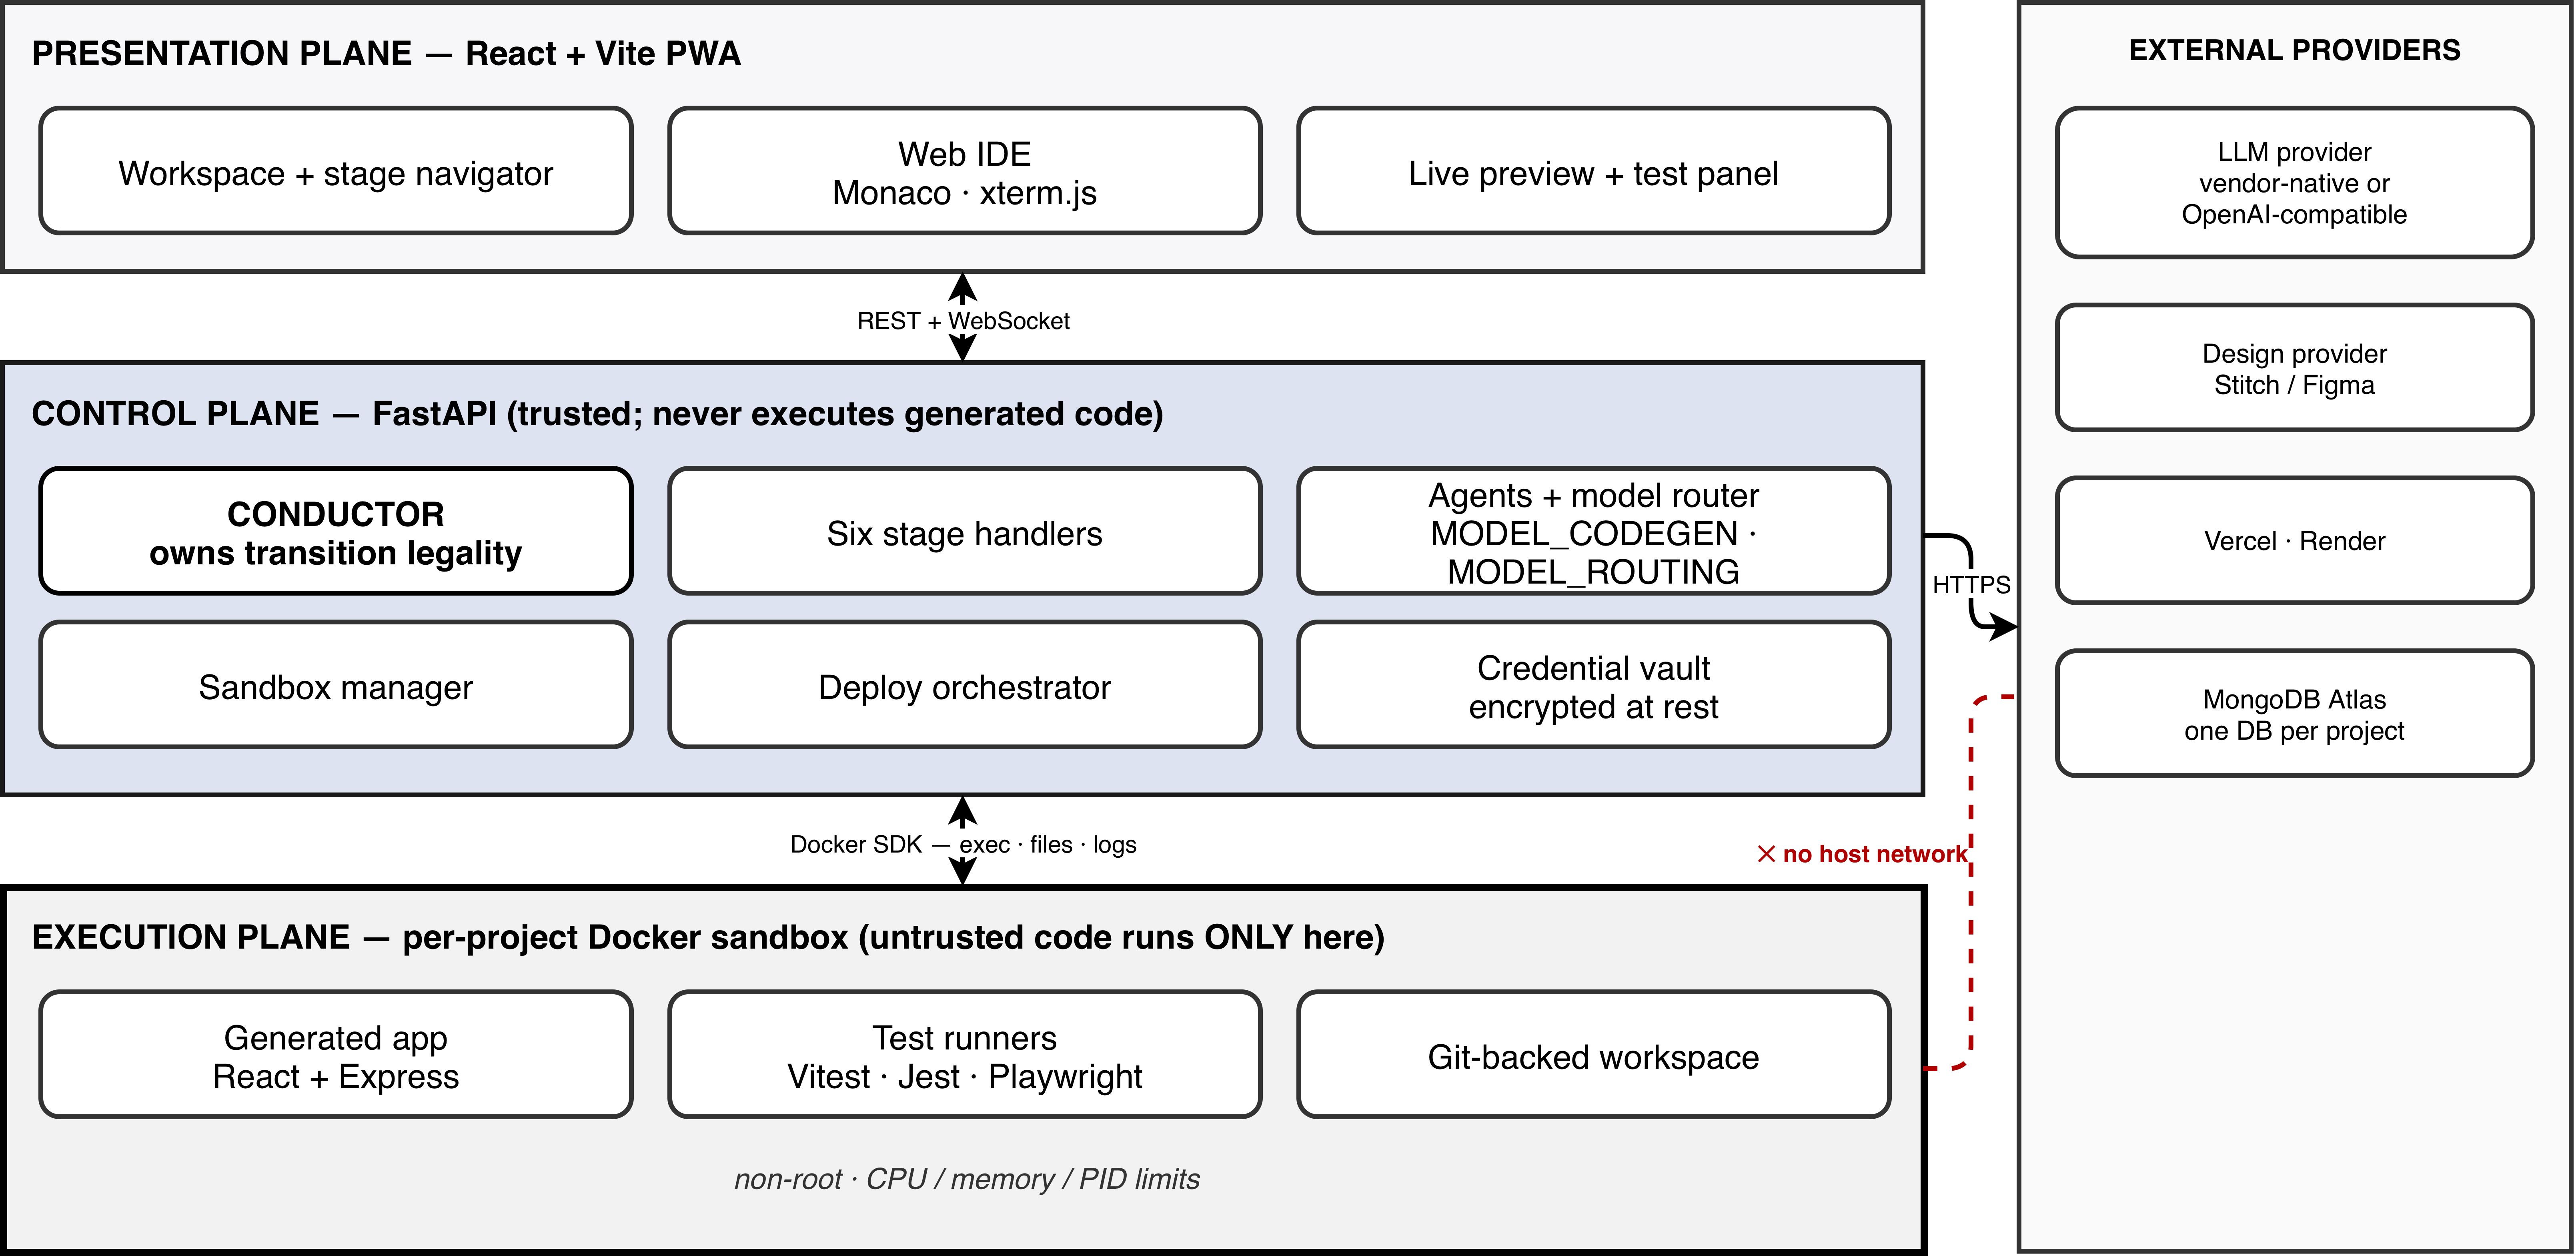
\includegraphics[width=\textwidth]{fig1.png}
\caption{ForgeFlow system architecture: the presentation, control and execution planes, and the external provider boundary. Untrusted generated code executes only inside the per-project sandbox, which has no host network.}\label{fig1}
\end{figure}

\subsection{Design Principles}\label{sec3.1}

\textbf{P1: Verification over generation.} The defensible contribution is knowing when the system is finished, not how quickly it emits code.

\textbf{P2: One fixed generated-app stack.} Every generated application is React (Vite + TypeScript) on the frontend, Node/Express (TypeScript) on the backend, and MongoDB via Mongoose, tested with Vitest, Jest + supertest, and Playwright. Constraining the target raises first-pass generation success, reduces the number of repair iterations required, and makes rigorous verification tractable within a student project's budget. It also lets a hand-written 53-file skeleton be \emph{copied} rather than generated, which removes scaffolding tokens entirely---the deterministic-scaffolding lesson of \cite{r13xia}.

\textbf{P3: Cost discipline as an architectural concern.} Model roles are separated, and model identifiers are configuration, not identity: a code-generation role (default claude-sonnet-5) for synthesis, repair and test generation, and a cheap routing role (default claude-haiku-4-5) for classification, summarisation and the freeform-description-to-feature-list draft. Every call records token usage against the project, and per-project and global budget caps halt work with an actionable message. This is a direct engineering answer to the ``high cost of correctness testing'' challenge named in \cite{r22pasuksmit}. A provider abstraction additionally allows any OpenAI-compatible endpoint to be substituted without touching agent, tool or cost code. The evaluation in Section~\ref{sec8} uses this path, with z-ai/glm-5.3-flash in both roles.

\textbf{P4: Never overwrite; always version.} Artifacts---designs, code changes, requirements, test suites, test runs, repair attempts, deployments, infrastructure plans---are versioned, never replaced, which is what makes ``revisit and refine'' safe.

\textbf{P5: Untrusted code runs only in sandboxes.} The control plane never executes generated code. Each project receives a Docker container running as a non-root user with no host network, dropped capabilities, and CPU, memory and PID limits, reaped when idle. Recent work on securing test environments for untrusted code documents how wide the escape surface of na\"{\i}vely configured execution environments actually is \cite{r24rabin}; ForgeFlow treats the sandbox boundary, not the model's good behaviour, as the security control.

\textbf{P6: Non-linearity is an invariant, not a feature.}

\subsection{Architecture}\label{sec3.2}

The structure of ForgeFlow is divided into three planes and an external provider boundary (Fig.~\ref{fig1}). The control plane is a FastAPI (Python 3.11) service that has Pydantic v2 schemas at all boundaries and Motor/Beanie on top of MongoDB. It includes authentication, project lifecycle and state of the project stages, the conductor, the six stage handlers, the agent layer, the sandbox manager, the deployment orchestrator, the encrypted credential vault, the evaluation harness, and a WebSocket hub. For every project a separate application database is created, and there is a forgeflow\_meta database for control plane metadata.

Each execution plane consists of a single Docker container that contains the workspace backed by Git, the generated application, the reverse-proxied preview of the application's development servers, and the test runners. The diff in Section~\ref{sec5} is not just a side-benefit of Git backing: It is what makes it computable.

The presentation plane is a PWA (Progressive Web App) installable using React 18: dashboard, a clickable stage navigator (workspace shell), a Monaco-based IDE that renders code as the agent writes it, an xterm.js terminal bridged to the sandbox shell, a live preview pane, a test-and-repair pane, a React Flow deployment topology, and a project data browser.

All work of long duration is event driven. A typed event has \{event, project\_id, stage, payload, seq\}; clients subscribe per project and resume from the previous seq after disconnect, so there is no loss of an in-flight generation/repair loop when the page is reloaded.

\subsection{The Non-Linear Stage Model}\label{sec3.3}

\begin{figure}[t]
\centering
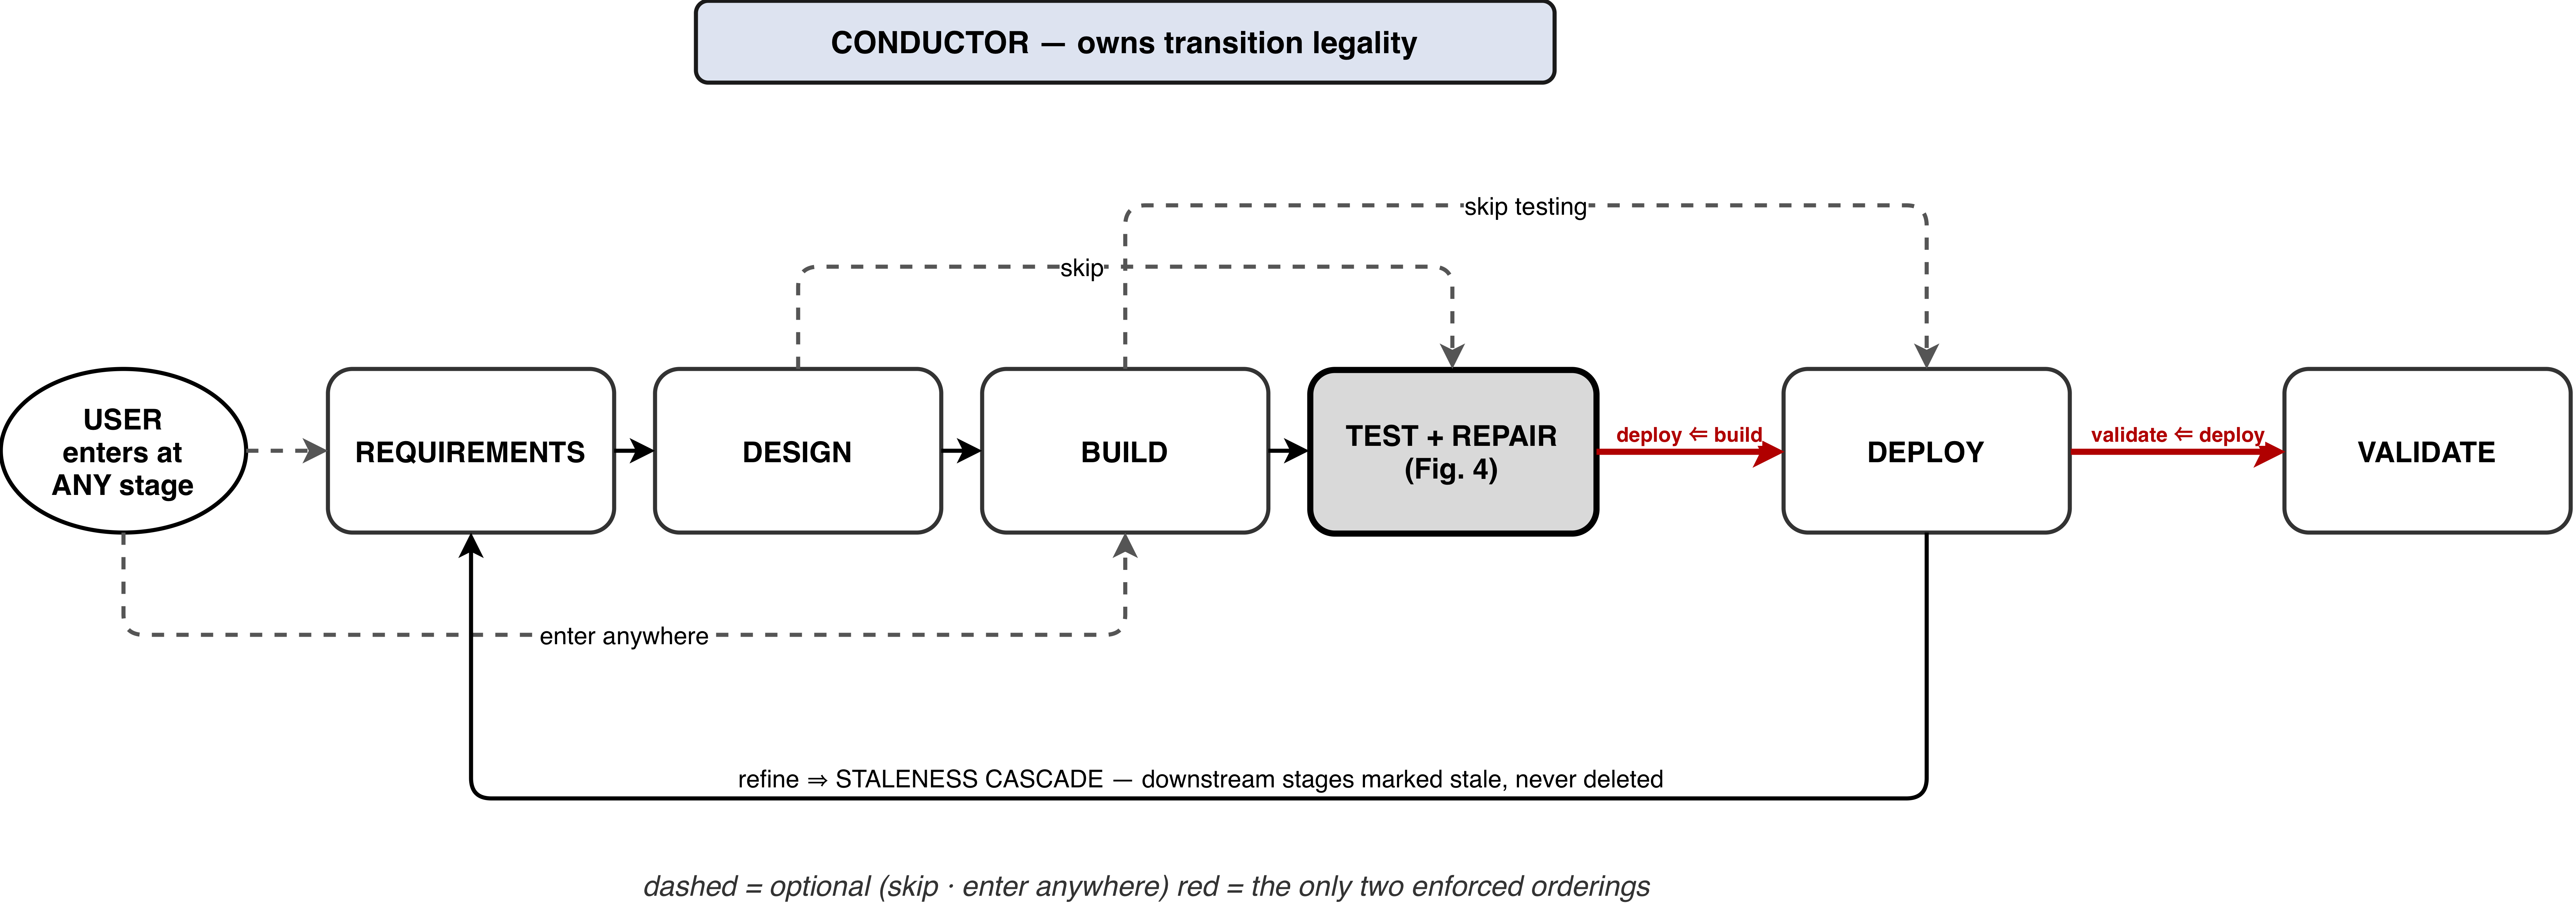
\includegraphics[width=\textwidth]{fig2.png}
\caption{The non-linear stage model. Dashed edges are not required (enter-anywhere and skip); the two bold edges are the only required orderings; artifacts in downstream edges are not deleted, but a staleness cascade is propagated.}\label{fig2}
\end{figure}

The flow of the product is requirements -- design -- build -- test -- deploy -- validate \chg{(Fig.~\ref{fig2})}. This order drives the navigator, the default entry stage and the staleness cascade and gates nothing.% [G30][K01] first citation of Fig. 2

One StageState is maintained for each project at each stage, and has statuses of \{empty, in\_progress, awaiting\_user, complete, skipped, stale\}. Three behaviours follow:

Enter anywhere. If a user has an existing design, he/she can begin at build, and if he/she has an existing workspace, he/she can begin at test.

Skip. Any stage can be skipped and each downstream handler must be able to accept missing artifacts from upstream handlers. No requirements are present when generating a test: warnings are issued and the test generation offers to capture the requirements or to infer a minimal set; it does not refuse.

Jump back and improve. If a stage is completed, re-entering it starts a new conversation round, outputs are new versions of artifacts, and any downstream stages are marked stale (not deleted) and remain inspectable and re-runnable.

Transition legality is the responsibility of the conductor, not the UI. It takes in an intent \{message, target\_stage, action $\in$ refine $\mid$ proceed $\mid$ skip \fix{$\mid$ unskip $\mid$ reset}\} and passes it to a stage handler, stores messages and artifacts, and sends out events. Centralising legality in one component is what keeps non-linearity a property of the system, and not one screen.% [FIX: D4 -- backend/app/orchestrator/schemas.py:80-97 IntentAction = refine|proceed|skip|unskip|reset]

Requirements precede design in the product order because a UI should not be designed before it is known what the application must do; when a specification exists, it is passed to the design provider's prompt as additional context. This is a soft nudge in the interface, not a gate, consistent with the human-control evidence in \cite{r07tang,r08huang}.

\section{Requirements-Driven Verification}\label{sec4}

\begin{figure}[t]
\centering
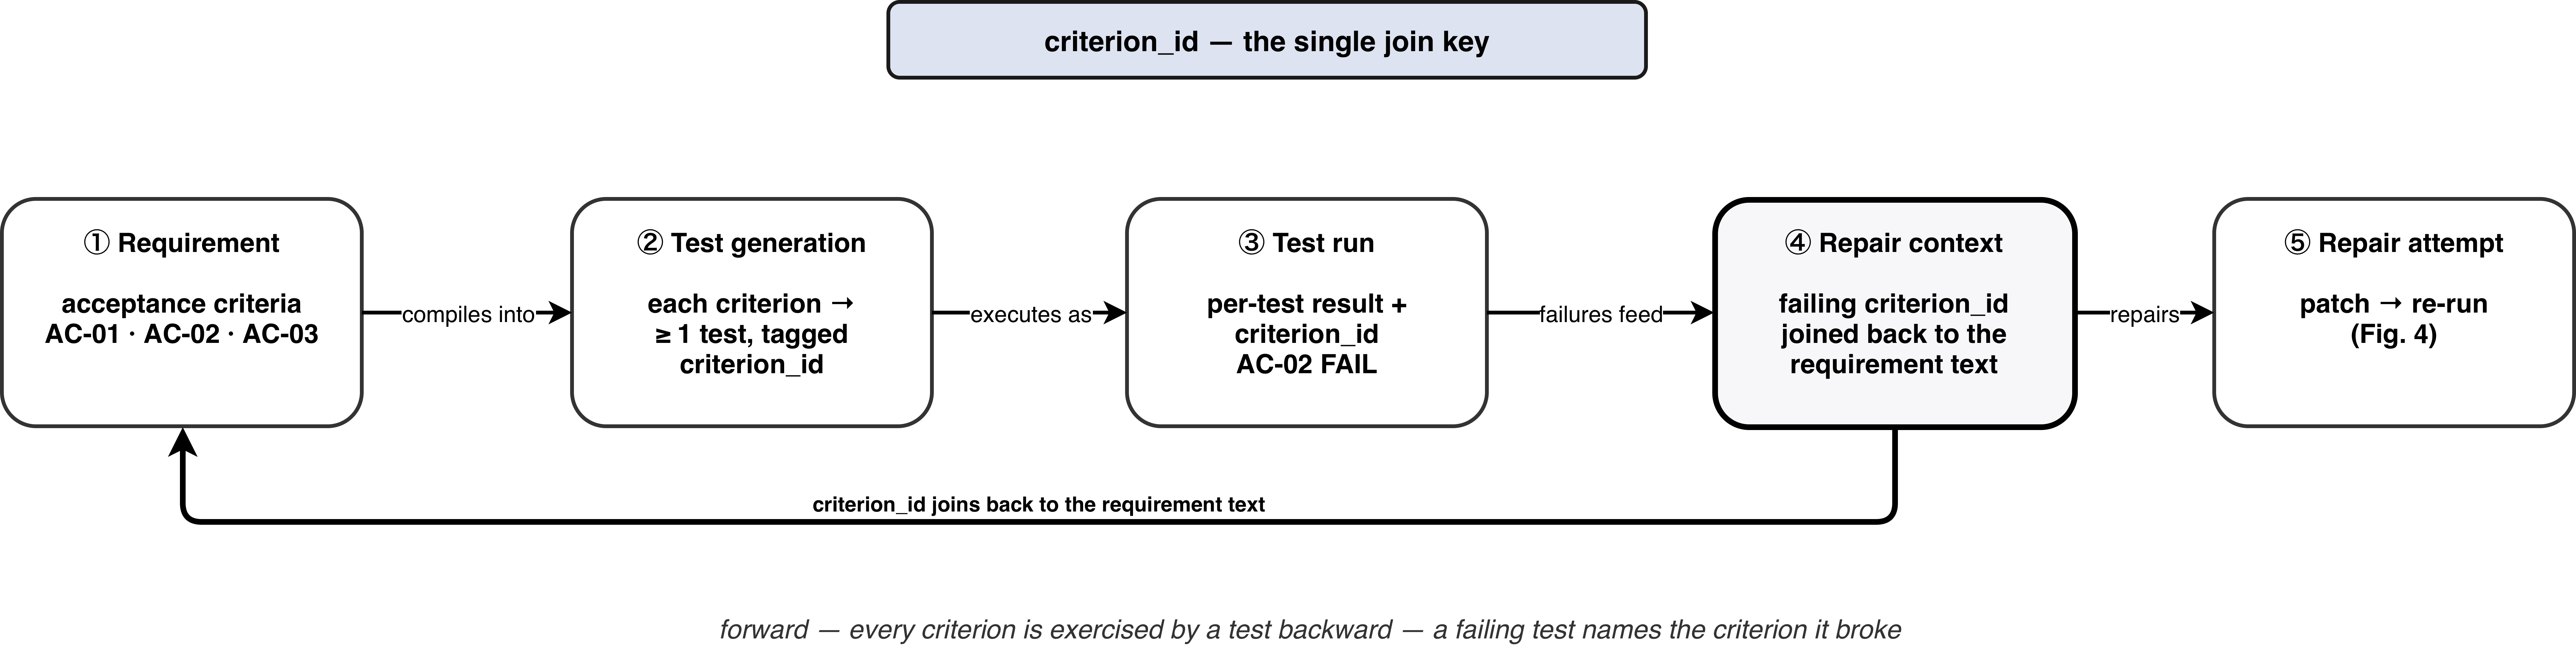
\includegraphics[width=\textwidth]{fig3.png}
\caption{The traceability chain. A user written acceptance criterion is passed through a single criterion\_id which are used to generate and execute tests, as well as to analyse failures and repair them, and are reattached to the requirement text when attempting a patch.}\label{fig3}
\end{figure}

\subsection{Structured Capture}\label{sec4.1}

A RequirementSpec contains a list of features, all of which have a name, description, set of inputs, expected behaviours, and acceptance criteria. Capture is not free prose, but is deliberately structured to get deterministic, evaluable test generation from it. They have two entry points: one guided and the other is an AI draft where a freeform description is translated into a proposed feature list by the routing model. The draft is never auto-saved, it is presented for editing and for following the human-control principle.

\subsection{Compilation to Executable Tests}\label{sec4.2}

The test-generation agent assigns each acceptance criterion to one or more executable test, each test being assigned with the identifier of the criterion that it tests \chg{(Fig.~\ref{fig3})}: Vitest and Testing Library for frontend units, Jest with supertest for backend units, Playwright for end-to-end behaviour exercised against the sandbox preview. This is very similar to the E2E derivation in \cite{r18alian} with the exception that an explicit identifier is added for traceability to persist in execution.% [G30][K01] first citation of Fig. 3

\subsection{Execution and Normalisation}\label{sec4.3}

Suites run in the project sandbox. The output of the \fixdel{JUnit and }JSON reporters are normalised to a per-test record \{status, assertion, stack, files\_referenced, criterion\_id\}. Three reasons for normalisation:% [FIX: D5 -- backend/app/testing/parsers.py:194-210 parses Vitest/Jest/Playwright JSON only; no JUnit parser]

\begin{enumerate}
\item The repair context in Section~\ref{sec5} is compiled deterministically from it.
\item A criterion that fails will not be included in an aggregate ``tests passed'' but will be reported as unmet.
\item The shape produced by the live validation run in Section~\ref{sec6} is the same, so that the repair path is framework agnostic.
\end{enumerate}

\section{The Bounded, Diff-Aware Self-Healing Repair Loop}\label{sec5}

\begin{figure}[t]
\centering
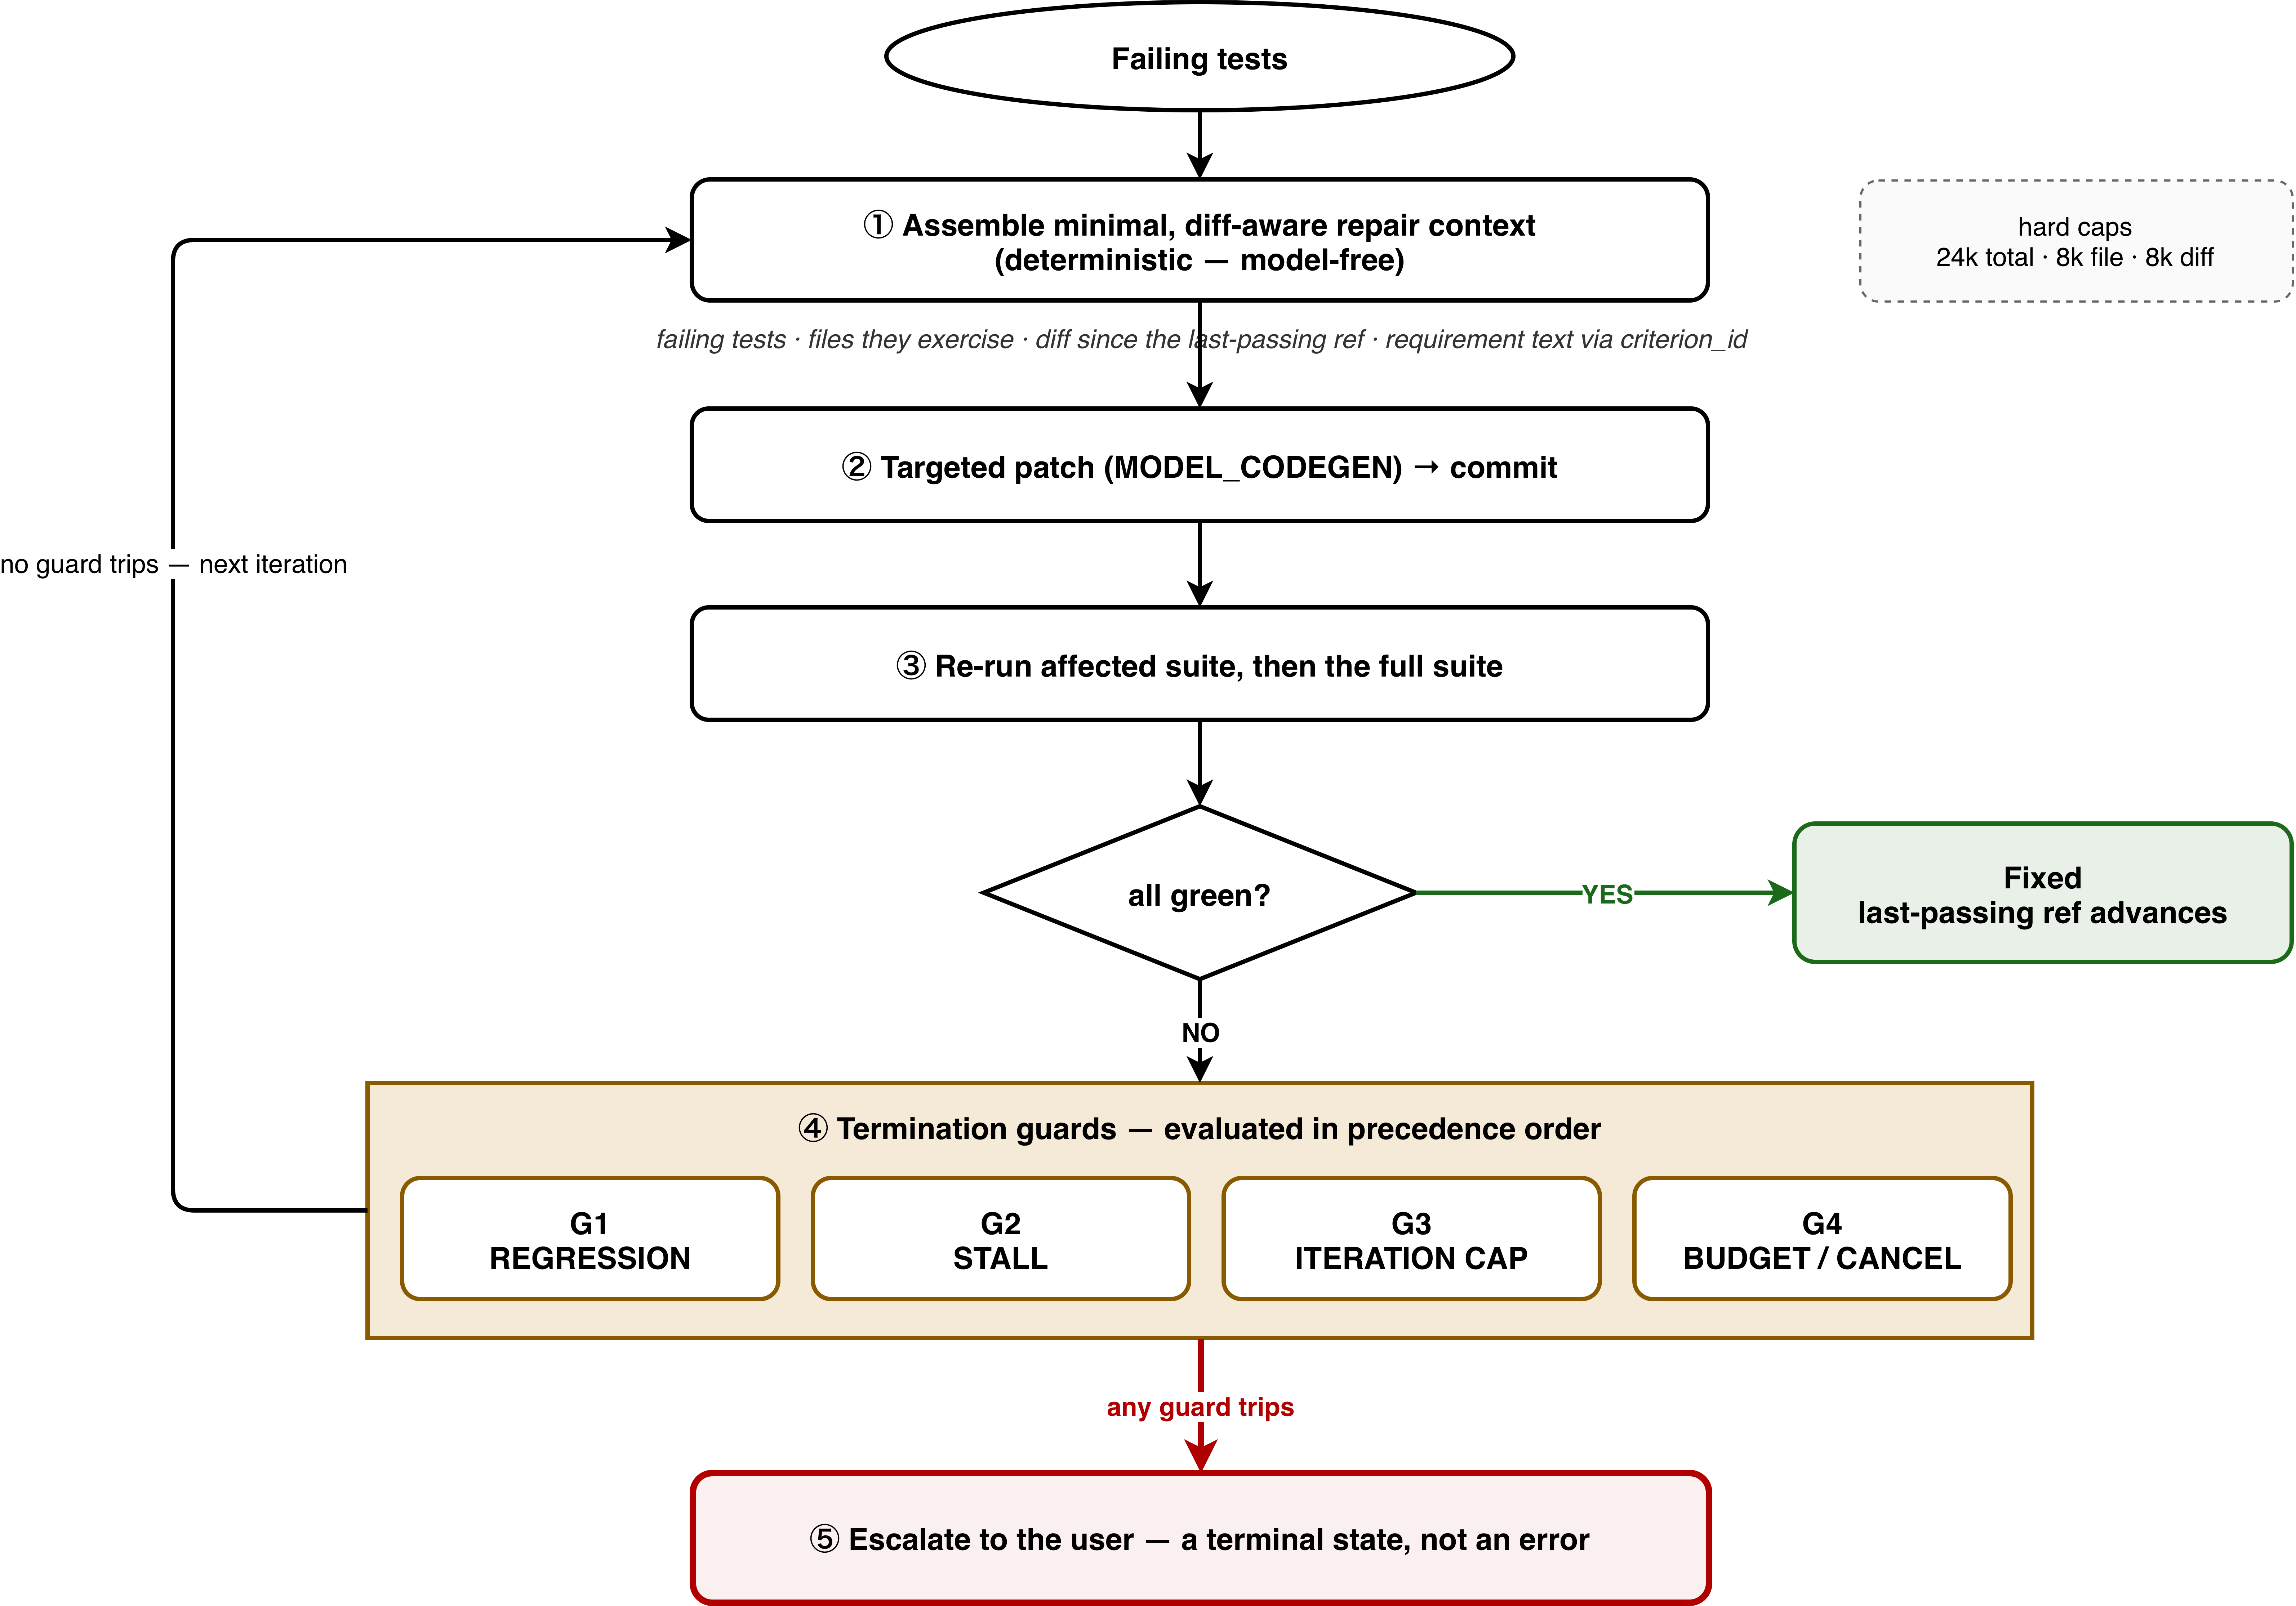
\includegraphics[width=\textwidth]{fig4.png}
\caption{The bounded self-healing repair loop: minimal context assembly, targeted patching, re-execution, termination guards in order of precedence, and escalation as terminal state.}\label{fig4}
\end{figure}

This is the core contribution \chg{(Fig.~\ref{fig4})}. It's given at least one TestRun that fails, the current workspace, and the requirements that the failing tests represent.% [G30][K01] first citation of Fig. 4

\subsection{Minimal, Diff-Aware Repair Context}\label{sec5.1}

The context assembly is deterministic, model free and is exhaustively testable. It allows only four things to be admitted:

\begin{enumerate}
\item Only the failing tests are listed here: name, framework, assertion, stack, referenced source files, and criterion\_id.
\item Only sources for those tests that fail: the failing test's source and files listed in the failing test's stack, widened along the failing test's import graph by a breadth-first walk bounded at depth 3 and 24 files. Package imports never resolve, so dependencies cannot enter the context, and the agent may request at most three further non-test files per attempt.
\item The difference between the current and last-passed line. This reference is moved: it is moved forward on each green run, not on the last commit, so the diff says ``what changed since it worked'', rather than ``what changed in the last commit.'' After observing that tests generated by this approach are not robust with respect to evolution and that models do not attend to presented code, this is the mechanism that \cite{r11haroon} recommends.
\item The requirement snippets for the failing criteria and a criterion\_id, to allow the agent to repair against the acceptance text instead of just the assertion.
\end{enumerate}

By construction, everything else is excluded (the rest of the repository, passing the tests, untouched modules). This result is capped (24\,000 characters total, 8\,000 per file, 8\,000 of diff, all run-time-configurable); parts that are too large are simply \fix{truncated or }dropped, and \fixdel{the number of times they are dropped}\fix{each one} is recorded, so a context which is too large is never silently lossy.% [FIX: D6 -- backend/app/agents/repair_context.py:237-240,298-306 truncate files/diff to their head, drop over-budget files, record each in `trimmed`]

\subsection{Targeted Patch and Re-execution}\label{sec5.2}

The repair agent only gets this context, and a hard constraint to repair the failing behaviour without breaking the passing tests. The patch is then put into the sandbox workspace and committed. The affected suite is rerun on the fast path and then rerun on the full path to check for regressions the fast path may not have discovered.

\subsection{The Loop Controller (Bounded Repair Controller)}\label{sec5.3}

Four guards terminate the loop, evaluated in a deliberate precedence order (defaults in parentheses; all admin-tunable):

\begin{itemize}
\item \textbf{Regression guard (2).} Trips on the second attempt that breaks a previously passing test. It is evaluated first because ``my patches keep breaking working code'' is a more precise and more actionable diagnosis than ``no progress''; a single regression is tolerated because a legitimate patch can briefly break one test. An attempt that broke something and fixed nothing is reverted, so the loop never hands back an application worse than it found.
\item \textbf{Stall guard (2).} Trips when the failing-test set has not shrunk for stall\_threshold consecutive iterations; a set that stays the same size counts as no progress, and any shrink resets the counter.
\item \textbf{Iteration cap (5).} Checked before each model call. The default sits just above the one-to-three-iteration range in which the literature finds most of the achievable gain \cite{r09kiecker,r10arimbur}, because further iterations are unproductive and can degrade security \cite{r05shukla}; Section~\ref{sec8.3} tests this choice.
\item \textbf{Budget, cancellation and blocked attempts.} The loop also ends when the budget cap is exhausted, the user cancels, the agent reports that nothing in its context is safe to patch, or two consecutive attempts write no file. A failure classified as a sandbox-environment fault escalates before any model call, at zero token cost. Every such ending is an escalation, never a crash.
\end{itemize}

Per attempt, RepairAttempt.outcome $\in$ \{fixed, no\_progress, regressed\} with regression dominating: an attempt that fixes one test and breaks another is still treated as dangerous.

\subsection{Escalation as a Terminal State}\label{sec5.4}

Each non-green ending resets the test phase to awaiting\_user and sends an event of type repair.escalation with the reason field containing the reason, a short summary of the current state ``here is where I am stuck'', a set of failed tests, diffs already tried, the convergence metrics, and an explicit resume contract (refine the Build stage with guidance, after which repair can run again). There is no error path to escalation. This is its encoded version of the invariant always prefer escalation over silent failure, and it is how the human-control pattern defined in \cite{r21takerngsaksiri} is extended to the repair phase.

\subsection{Audit Trail and Convergence Metrics}\label{sec5.5}

Each iteration is persisted as a RepairAttempt containing its target files, diff reference, resulting run and whether it was reverted, and the whole loop is persisted as one costed Run with outcome \{fixed, escalated\}. A versioned repair report captures initial\_failing, final\_failing, failing\_by\_iteration[], regressions\_introduced, empty attempts, iterations, tokens\_spent, cost\_inr and wall\_clock\_s, and repair.iteration \{i, failing\_count, regressions, tokens\} events stream to the UI while the loop runs. This report is also the unit that the evaluation harness consumes (Section~\ref{sec8}).

The loop's invariants are: If a diff will do, do not feed the whole repository; If the loop will not terminate, bail out; Always leave an auditable trail; Always prefer escalation to silent failure.

\section{Deployment and Live Validation}\label{sec6}

\begin{figure}[t]
\centering
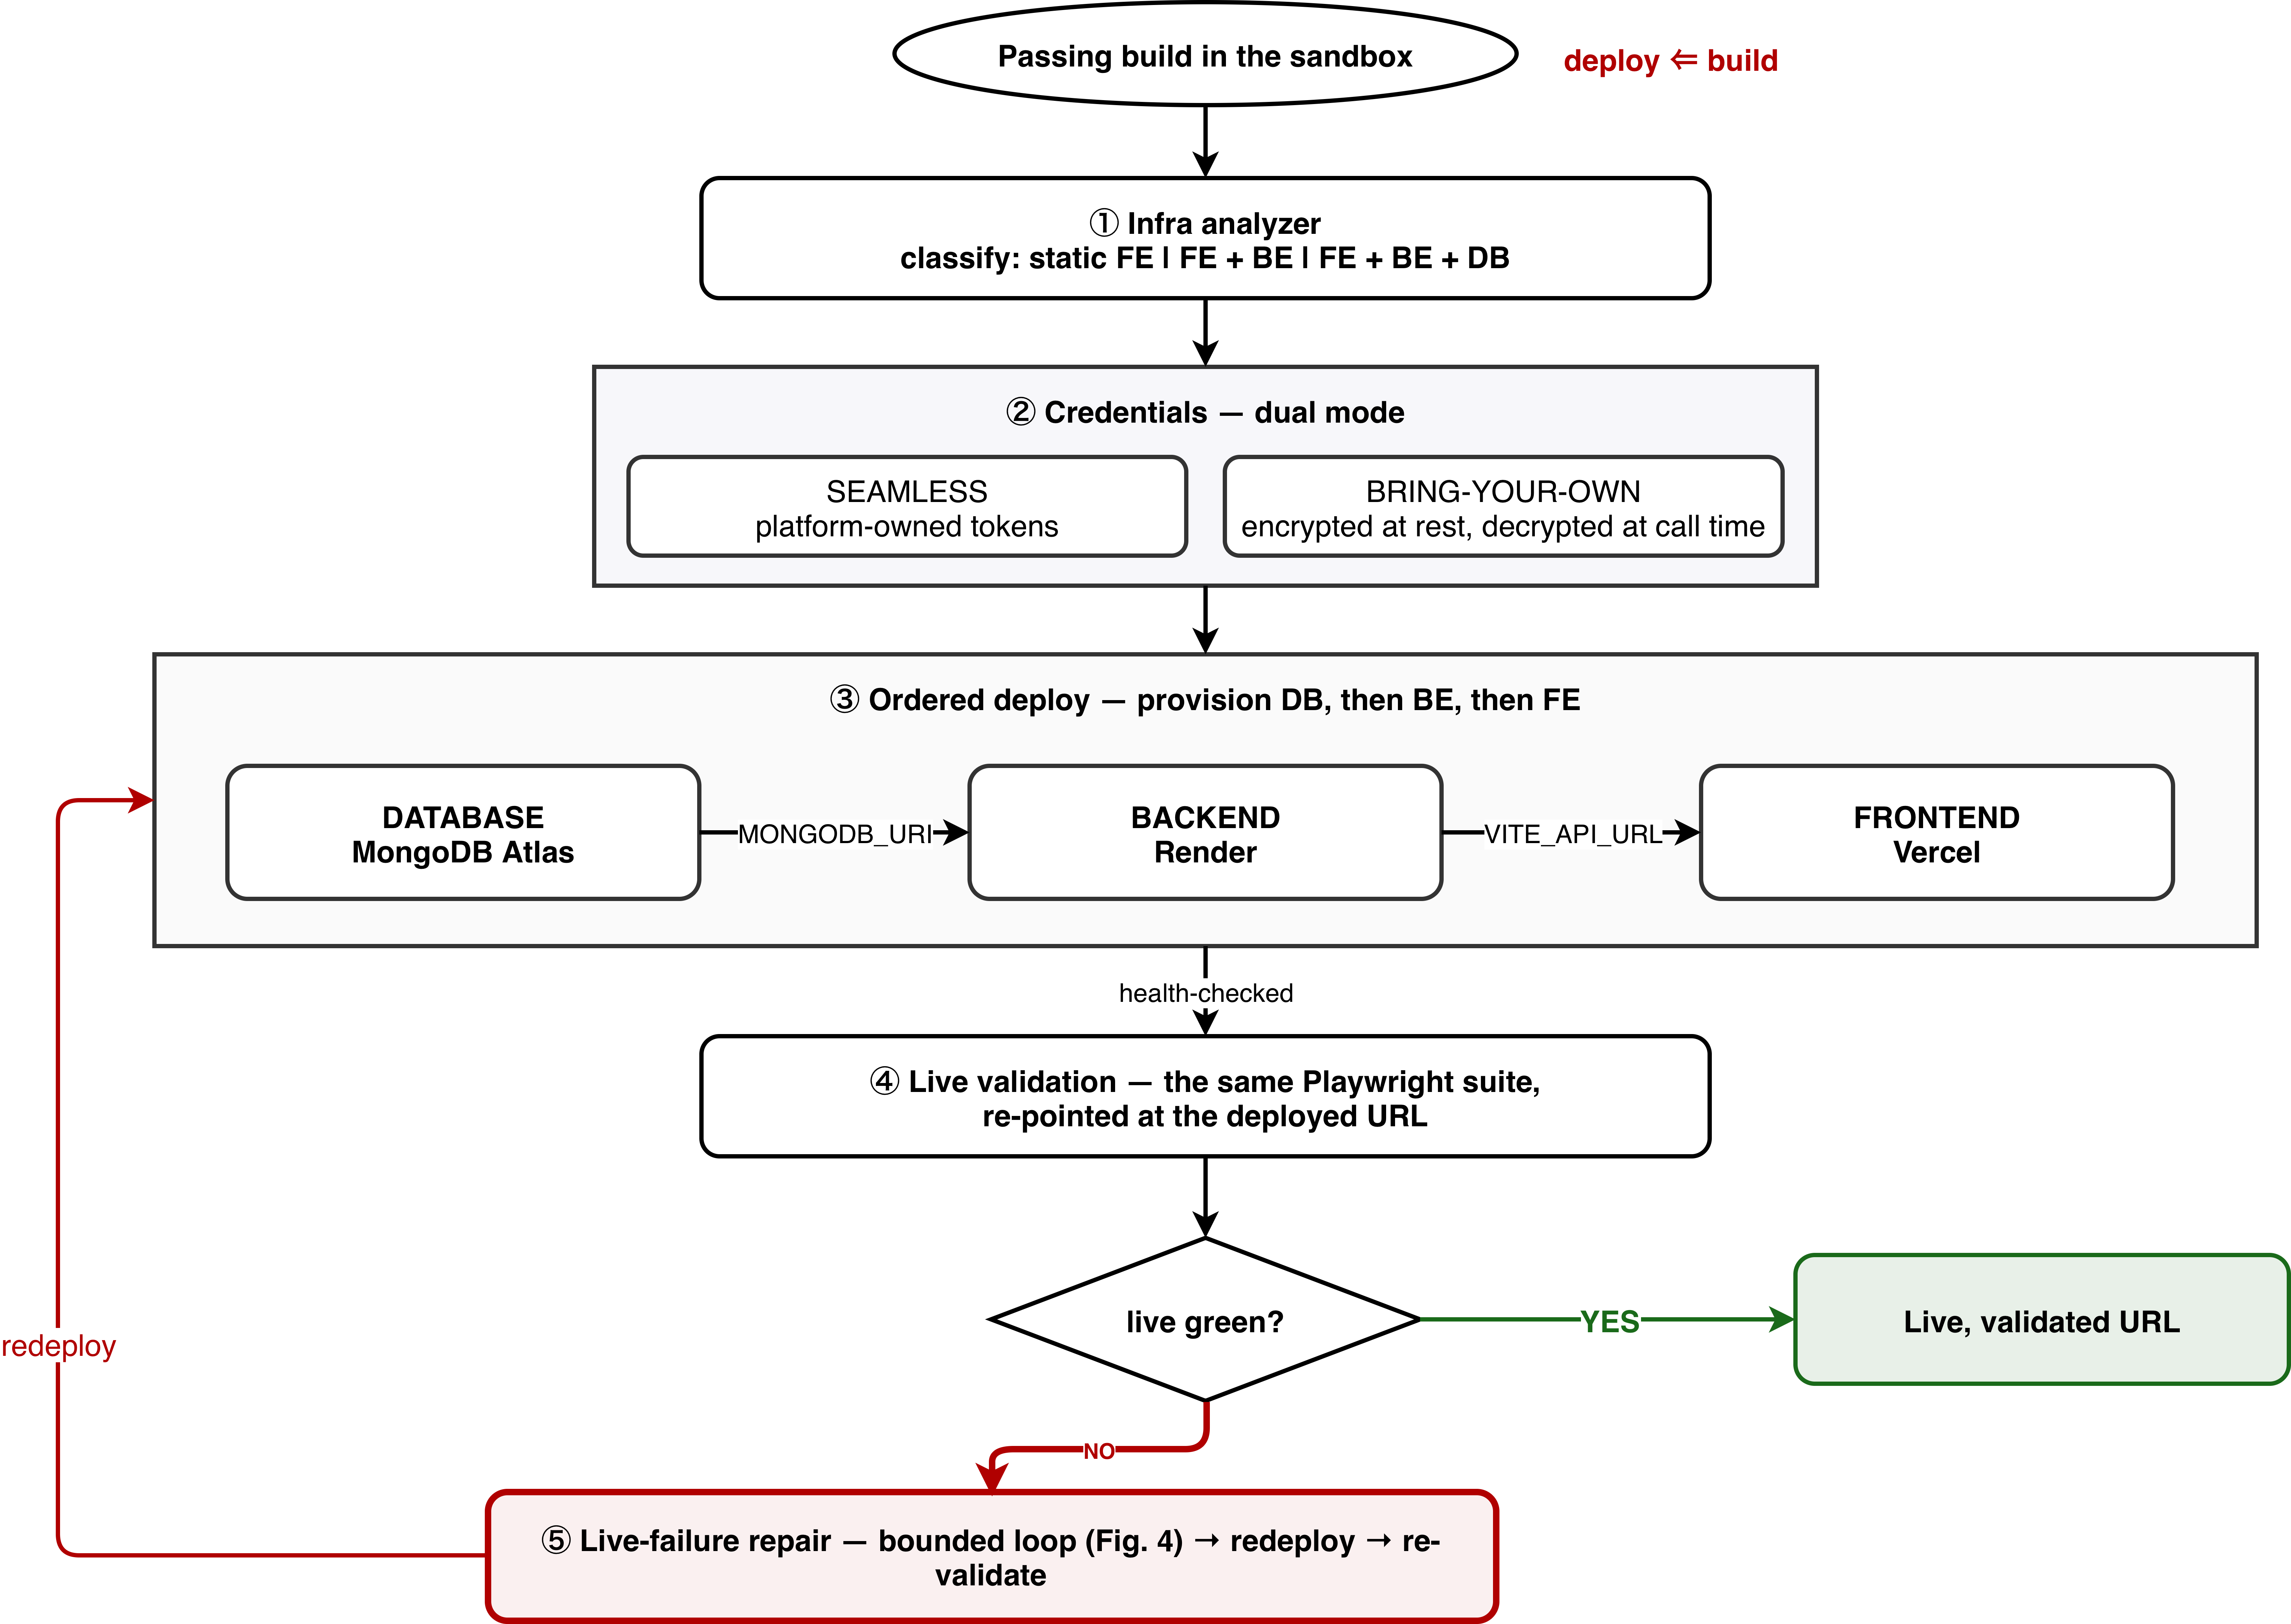
\includegraphics[width=\textwidth]{fig5.png}
\caption{The infrastructure analysis, dual mode credential handling, topology for deployment, and the path for live failure repair and validation after deployment. The figure shows the original Render backend; the backend now deploys to Vercel by default, with Render available as an option.}\label{fig5}
\end{figure}

\subsection{Infrastructure Analysis}\label{sec6.1}

An analyser will analyse the workspace; frontend build target, whether or not a persistent backend will be attached, whether or not a database will be used and what type, required environment, etc.; and produce an infra\_plan artefact that identifies the project as a static frontend, or a frontend with a persistent backend, or a frontend with a backend and a database, with recommended build targets and exact environment variables and secrets each needs \chg{(Fig.~\ref{fig5})}. The motivation given in \cite{r06zhang} is a 30.2~\% / 26.8~\% first-attempt deployment success rate; deployment configuration is a failure mode beyond the scope of generation quality.% [G30][K01] first citation of Fig. 5

\subsection{Dual-Mode Credentials and Ordered Deployment}\label{sec6.2}

There are two ways to deploy: Seamless, which is deployed on the provider account that hosts the platform; or Bring Your Own, which is deployed with the user's own tokens. All provider tokens are encrypted at rest using Fernet, and will only be decrypted at call time, in process, and are never logged and never returned to the client. Both tiers deploy to Vercel---the SPA as static assets and the Express backend as a function---from the same inline file upload, so no git host is involved and what ships is exactly what the repair loop validated; Render remains available for the backend as an option. Deployment is ordered: provision the database; deploy the backend with the database URI injected; deploy the frontend with the backend's public URL injected; and health-check every node, so a dead backend never ships behind a live frontend. A pre-flight check refuses a localhost database URI before anything is deployed. The resulting topology is depicted as an interactive React Flow graph with per-node status, logs and redeploy controls.

\subsection{Post-Deployment Validation}\label{sec6.3}

It is then re-pointed to the deployed URL with the same Playwright suite. As the live run yields the same normalised shape as in-sandbox, upon failure, the live run re-enters the same repair loop as the in-sandbox run, which is Section~\ref{sec5}: diagnose, repair, redeploy, re-validate. Live failures get at most two repair, redeploy and re-validate cycles. This closes the loop on the artifact the user will actually use, a step that none of the other system classes in Table~\ref{tab1} performs.

\section{Implementation}\label{sec7}

\begin{figure}[t]
\centering
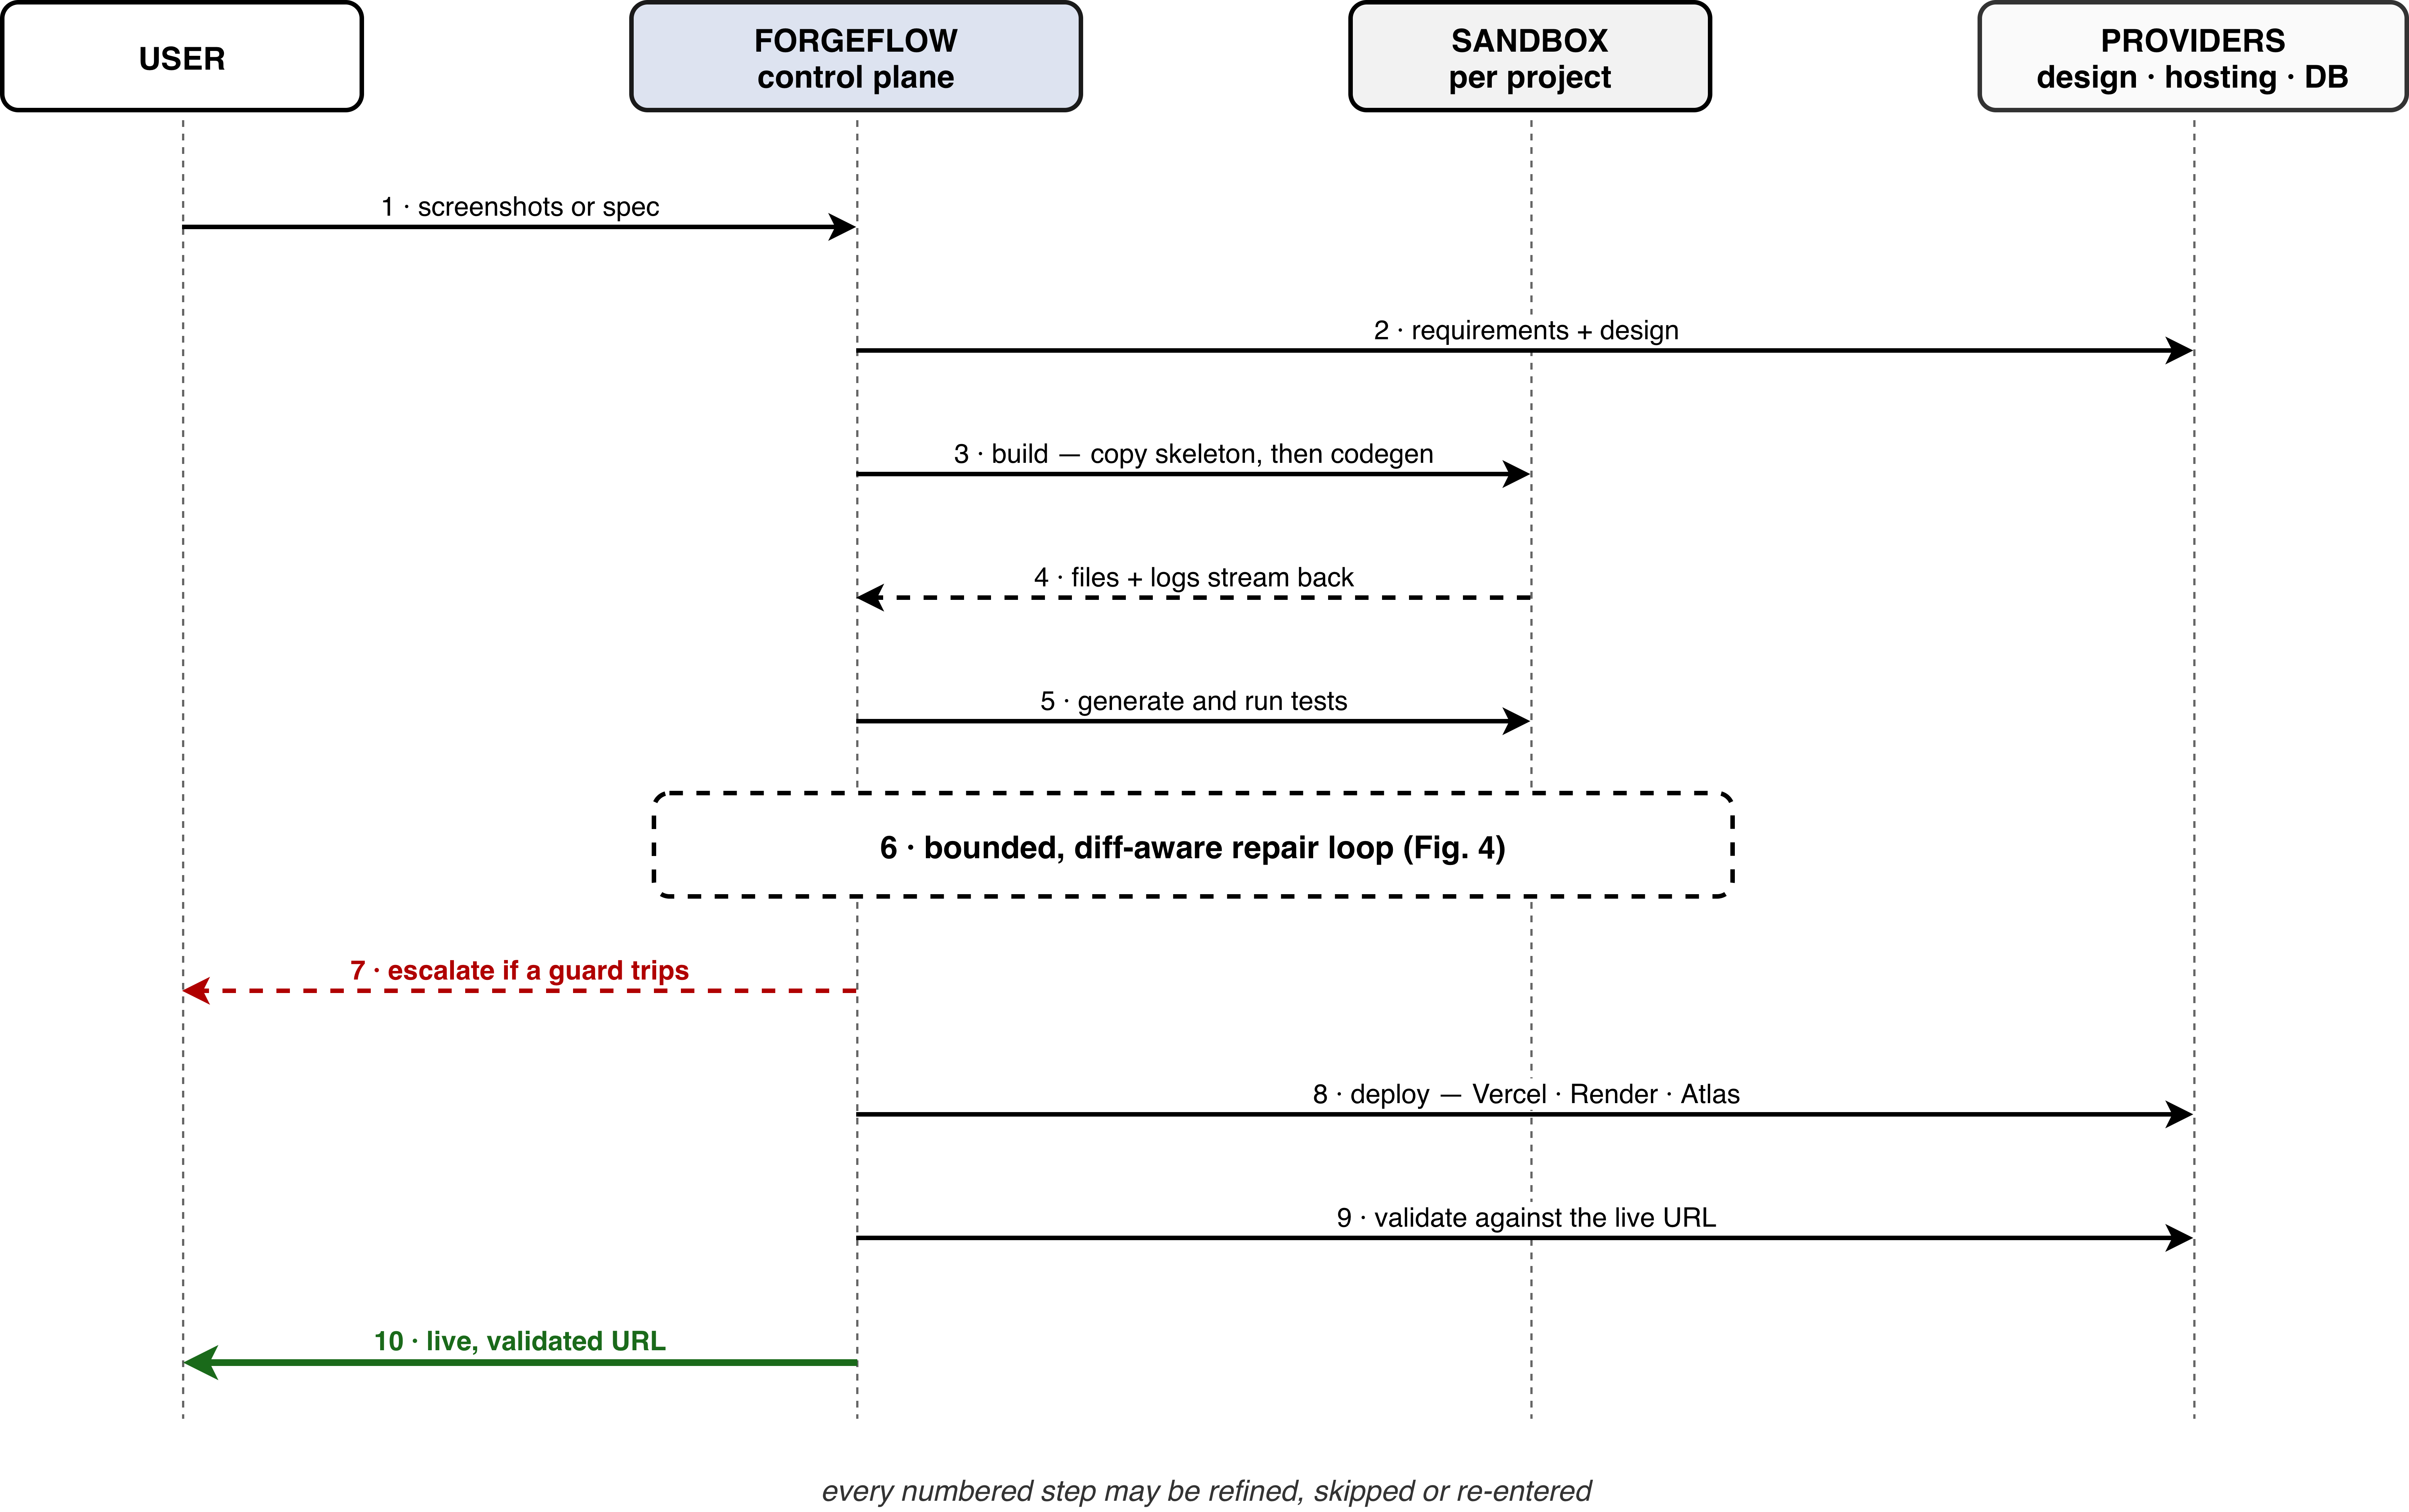
\includegraphics[width=\textwidth]{fig6.png}
\caption{The end-to-end hero path, from screenshot or specification intake to a live URL validated against production. Every numbered step remains refinable, skippable and re-enterable.}\label{fig6}
\end{figure}

A complete prototype has been implemented across \fixdel{65}\fix{67} independently shippable phases grouped into 14 epics, each phase gated on its own acceptance criteria and tests before being marked done \chg{(Fig.~\ref{fig6})}. Table~\ref{tab2} summarises its scale, measured from the repository on 4 October 2026 (physical lines of non-test source).% [FIX: D2 -- plans/README.md at commit c5a7835 (4 Oct 2026) lists 67 phases (01-67, all done) in epics 0-13] [G30][K01] first citation of Fig. 6

\begin{table}[t]
\caption{Implementation Scale of the ForgeFlow Prototype}\label{tab2}%
\small
\begin{tabular*}{\textwidth}{@{\extracolsep\fill}p{3.9cm}llp{3.5cm}@{}}
\toprule
\raggedright{}\textbf{Component} & \textbf{Modules} & \textbf{Lines of code} & \raggedright{}\textbf{Automated tests}\tabularnewline
\midrule
\raggedright{}Control plane (FastAPI, Python 3.11) & 175 & 35\,426 & \raggedright{}1\,815 tests / 234 files\tabularnewline
\raggedright{}Frontend PWA (React 18 + TypeScript) & 133 & 18\,452 & \raggedright{}508 tests / 61 files\tabularnewline
\raggedright{}Generated-app skeleton (fixed stack) & 53 files & --- & \raggedright{}placeholder suites (FE/BE/E2E)\tabularnewline
\raggedright{}\textbf{Total production code} & \textbf{308} & \textbf{53\,878} & \raggedright{}\textbf{2\,323 automated tests}\tabularnewline
\raggedright{}Test code & 295 files & 46\,169 & \raggedright{}---\tabularnewline
\raggedright{}Benchmark specifications & 10 YAML specs & --- & \raggedright{}---\tabularnewline
\botrule
\end{tabular*}
\end{table}

\textbf{Test-suite performance.} In the full-suite run of 2 October 2026 all 2\,253 executed tests passed and none failed: 1\,745 backend tests in 653 s and 508 frontend tests in 167 s. The other 70 backend tests are skipped by design on the development host (66 POSIX-only, 4 opt-in tests needing Docker or the real pnpm toolchain) and run on the Linux CI runners.

Notable Implementation Properties:

\begin{itemize}
\item \textbf{Layered configuration.} More than 100 runtime settings resolve with precedence; they are admin panel $>$ environment $>$ default and include the repair caps and the stall thresholds; the behaviour of the loop can thus be adjusted from an administrative dashboard and tested by the evaluation harness without redeployment. At the interface, it's write-only as well, and it's encrypted at rest with Fernet encryption - the encryption key and the control-plane database URI are still in the environment, since they're read before the configuration layer exists and protect the ciphertext itself.
\item \textbf{Quality gates.} TypeScript is strict with ESLint and Prettier rules; the Python codebase is ruff, black and mypy clean, with full type hints and no bare exception handling. Errors are grouped into a single taxonomy that distinguishes between user and system and provider errors and provider degradation, notably design-provider quota exhaustion, is handled softly with an actionable message and a fallback, while no longer terminating the pipeline.
\item \textbf{Security posture.} All authorisation is enforced per route; no cross-project data access is available; generated code never runs in the control plane; the sandbox doesn't have a host network and has dropped capabilities. This is done on purpose because of the credential- and error-handling smell classes reported for AI-generated infrastructure code in \cite{r04ghammam} and the execution-environment vulnerabilities enumerated in \cite{r24rabin} are located in the platform, not the prompt.
\item \textbf{Delivery and rollback.} The platform is itself delivered by a six-job CI pipeline and health-checked continuous deployment. On a k3s cluster probed every 0.2 s, a rolling update, a deliberately broken release and its automatic rollback served 807 requests with zero failures; the broken release served none.
\end{itemize}

\section{Evaluation}\label{sec8}

\subsection{Questions and Set-up}\label{sec8.1}

The evaluation addresses three questions. RQ1: does the bounded repair policy improve on a no-repair baseline, and at what cost and latency? RQ2: how is the gain distributed over iterations, and is the default cap of five justified? RQ3: on whole applications, how many acceptance criteria are met, and is every failure accounted for by the system's own explanations? All numbers come from one reproducible command (make eval), run on 2 October 2026.

Level 1 runs four industry benchmarks through ForgeFlow's own LLM transport and repair policy: HumanEval (164 Python problems) \cite{r25chen}; the sanitised test split of MBPP (257) \cite{r26austin}; HumanEval-TS, the TypeScript translation of HumanEval from MultiPL-E (159) \cite{r27cassano}, which matches the language of the generated applications; and BFCL v3 \cite{r28patil} (1\,000 non-live AST cases in four categories plus 240 irrelevance cases), whose function calls mirror the agents' tool use. Level 2 runs benchmark applications through the full pipeline (requirements, build, test generation, test and repair), each in its own project, sandbox and database. All runs used one model, z-ai/glm-5.3-flash, through an OpenAI-compatible endpoint (OpenRouter) pinned to the model developer's own upstream with fallback disabled, so every call was served by the same deployment; code generation used temperature 0 and BFCL 0.001.

\textbf{Baseline and repair policy.} The baseline is pass@1 on the same problems, model and grader, i.e. the no-repair arm. For each first-attempt failure, the repair arm returns the task, the current code and the last 1\,500 characters of the failing output to the model---not a growing transcript---for at most five attempts, and stops after two consecutive attempts that reproduce the same failure or resubmit known code: the product defaults max\_iterations = 5 and stall\_threshold = 2. As in the self-repair literature \cite{r29chen,r30olausson}, feedback comes from the benchmark's own tests, so the post-repair figure measures what repair adds and is not a pass@1 result. Function-level problems have no repository history, so Level 1 exercises the bounded controller but not the diff and import-graph parts of the context; \fixdel{those are}\fix{the diff can be} exercised only at Level 2\fix{, and the import-graph walk at neither level}.% [FIX: D3 -- backend/app/eval/runner.py:195 builds RepairLoopController() whose default analyzer (orchestrator/stages/repair.py:224, agents/repair_context.py:212 computes the diff) has no import-graph walk; that widening (SuiteRepairContextAnalyzer) is used only by the product's Test-stage repair (testing/repair_router.py:107); the recorded Level-2 run had no green run (no last-passing ref, so no diff) and made 0 repair attempts]

\subsection{Metrics and Their Validation}\label{sec8.2}

Table~\ref{tab3} defines each metric and states how it was validated. Before any model output was scored, the graders were checked: 426 of 426 reference solutions (upstream references for HumanEval and MBPP plus five hand-written TypeScript controls) pass, and 580 of 580 deliberately wrong stubs are rejected. Each dataset is pinned to an upstream commit \fix{(HumanEval-TS by content hash)} and verified by SHA-256 before use, and model-written code runs only in a container with no network, all Linux capabilities dropped, a read-only root file system and memory, CPU and process limits. The evaluation harness, including its metric pipeline, is covered by 130 unit tests. Proportions are reported with 95\% Wilson score intervals \cite{r31wilson}, and paired before/after outcomes on the same problems are compared with an exact McNemar test \cite{r32mcnemar}.% [FIX: D8 -- backend/app/eval/bench/datasets.py:36-42 MultiPL-E HumanEval-TS "cannot be pinned to a revision ... pinned by content hash"]

\begin{table}[t]
\caption{Metrics, Definitions and Validation}\label{tab3}%
\small
\begin{tabular*}{\textwidth}{@{\extracolsep\fill}p{2.2cm}p{5.2cm}p{4.3cm}@{}}
\toprule
\raggedright{}\textbf{Metric} & \raggedright{}\textbf{Definition} & \raggedright{}\textbf{Validation}\tabularnewline
\midrule
\raggedright{}pass@1 & \raggedright{}Solved by one greedy sample, graded only by the benchmark's tests & \raggedright{}426/426 references pass; 580/580 wrong stubs rejected; SHA-256-pinned data\tabularnewline
\raggedright{}Post-repair rate & \raggedright{}Solved within $\leq 5$ attempts given task, code and failing output; not a pass@1 & \raggedright{}Same grader; stop reason recorded per item\tabularnewline
\raggedright{}Repair conversion & \raggedright{}Repaired $\div$ first-attempt failures & \raggedright{}Exact McNemar test vs.\ no-repair baseline\tabularnewline
\raggedright{}BFCL accuracy & \raggedright{}Call matches a possible answer (AST); irrelevance = no call & \raggedright{}Official checker port; every failure typed\tabularnewline
\raggedright{}Criterion met & \raggedright{}$\geq 1$ tagged test ran and none failed; untested = unmet & \raggedright{}Criterion coverage reported (16/16)\tabularnewline
\raggedright{}Delivered & \raggedright{}All tests pass and all criteria met & \raggedright{}---\tabularnewline
\raggedright{}Latency & \raggedright{}Wall-clock per item, first request to verdict, incl.\ sandboxed execution; per stage for apps & \raggedright{}Monotonic clock; excludes queueing\tabularnewline
\raggedright{}Cost & \raggedright{}Tokens $\times$ list price (INR) & \raggedright{}Upper bound: cache discounts ignored\tabularnewline
\botrule
\end{tabular*}
\end{table}

\subsection{Code Generation and the Iteration Budget}\label{sec8.3}

Table~\ref{tab4} and Fig.~\ref{fig7}(a) give the results (RQ1). Bounded repair converted 13 of 19 first-attempt failures (68\%), raising pass rates by 1.3 to 2.7 percentage points. Because problems that pass first are never re-attempted, every discordant pair favours repair; the pooled exact McNemar test gives $p = 0.00024$, but per benchmark the gain is significant only for MBPP ($p = 0.016$), and the per-benchmark confidence intervals overlap. The effect is real but small because the baseline is already near its ceiling. Repair added 33 model calls to the 580 first-attempt calls (+5.7\%).

\begin{table}[t]
\caption{Code Generation: pass@1 Versus Bounded Repair (One Run, Temperature 0)}\label{tab4}%
\small
\begin{tabular*}{\textwidth}{@{\extracolsep\fill}lcccc@{}}
\toprule
\textbf{Measure} & \textbf{HumanEval} & \textbf{MBPP} & \textbf{HumanEval-TS} & \textbf{Pooled} \\
\midrule
Problems & 164 & 257 & 159 & 580 \\
pass@1, \% & 97.0 & 96.1 & 97.5 & 96.7 \\
95\% CI & 93.1--98.7 & 93.0--97.9 & 93.7--99.0 & 94.9--97.9 \\
After repair, \% & 99.4 & 98.8 & 98.7 & 99.0 \\
95\% CI & 96.6--99.9 & 96.6--99.6 & 95.5--99.7 & 97.8--99.5 \\
Gain, pp & +2.4 & +2.7 & +1.3 & +2.2 \\
Repaired / failed first & 4/5 & 7/10 & 2/4 & 13/19 \\
Mean attempts per repair & 1.25 & 1.29 & 1.00 & 1.23 \\
Stopped by stall guard & 1 & 3 & 2 & 6 \\
Exact McNemar $p$ & 0.125 & 0.016 & 0.500 & 0.00024 \\
Median / p95 latency, s & 13.5 / 73.8 & 7.6 / 68.0 & 11.6 / 93.8 & 10.6 / 78.4 \\
Model calls & 171 & 275 & 167 & 613 \\
Tokens (thousands) & 358 & 471 & 332 & 1\,161 \\
Cost, INR & 14.74 & 19.82 & 13.59 & 48.15 \\
\botrule
\end{tabular*}
\end{table}

\textbf{Iteration budget.} Fig.~\ref{fig7}(b) reconstructs the outcome under smaller caps by truncating each recorded trajectory (RQ2); this is exact for the recorded run, because a cap never changes the attempts before it. Ten repairs succeeded at the first attempt and three at the second, so any cap of two or more recovers all 13 and a cap of one recovers ten. The six unrepaired problems stopped on the stall guard after two to four attempts, and none reached the cap. Without the stall guard they could have run to the cap, consuming up to 46 attempts instead of 33, at the price of not observing whether a late attempt would have succeeded. At function level the knee is therefore at one to two iterations, consistent with \cite{r09kiecker,r10arimbur}; the cap of five was never binding, and the stall guard did the bounding.

\begin{figure}[t]
\centering
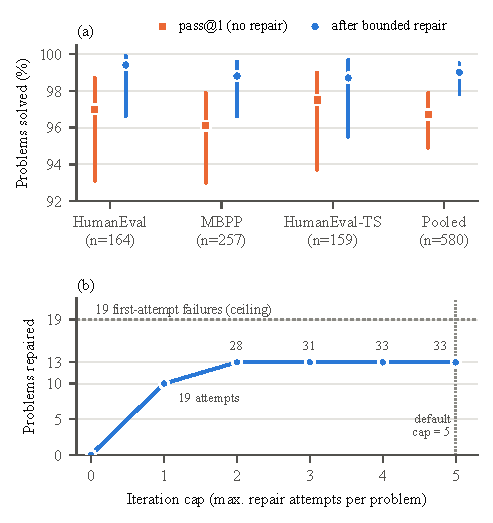
\includegraphics[width=0.6\textwidth]{fig7.pdf}
\caption{Function-level repair results on HumanEval, MBPP and HumanEval-TS. (a) pass@1 and post-repair pass rate with 95\% Wilson intervals. (b) Problems repaired, out of 19 first-attempt failures, for iteration caps 0--5, reconstructed from the recorded trajectories; the numbers by the points are the total repair attempts spent.}\label{fig7}
\end{figure}

\textbf{Latency and cost.} Median per-problem latency was 10.6 s (p95 78.4 s), but the distribution is heavy-tailed: first-attempt passes took a median of 10.4 s (p95 56.9 s), repaired problems 264.9 s and unrepaired problems 894.9 s (maximum 1\,424.7 s). The 19 first-attempt failures (3.3\% of problems) consumed 49\% of total problem time and the six unrepaired ones alone 29\%: failures, not successes, dominate wall-clock time, which is the practical case for stopping early. Reasoning tokens made up 85\% of output tokens, which explains both the tail and most of the cost. With eight problems in flight per suite \fix{(twelve for BFCL)}, the four benchmarks took 110 min, 1\,853 model calls and INR 64.58; costs are list-price upper bounds.% [FIX: D9 -- backend/app/eval/bench/code.py:218 concurrency=8; backend/app/eval/bench/bfcl.py:397 concurrency=12]

\subsection{Tool Calling}\label{sec8.4}

On BFCL (Table~\ref{tab5}), mean accuracy over the four AST categories was 92.7\%, with a median latency of 21.5 s per case (p95 29.6 s). All 141 failures carry a checker-assigned type: 75 (53\%) are calls made where no offered function fits; 45 are structural errors in multi-call cases (23 with the wrong number of calls, 22 with a call that matches no expected answer); 15 are argument values outside the allowed set; and 6 are type, unknown-function or missing-call errors. The irrelevance accuracy of 68.8\% is the clearest weakness: in about 31\% of such cases the model acts where it should abstain. ForgeFlow does not rely on the model abstaining; approval points, awaiting\_user states and escalation are the structural mitigation. The mean covers only the Python non-live categories and is not comparable with the leaderboard's overall score.

\begin{table}[t]
\caption{BFCL v3 Non-Live (Python) Accuracy, Official AST Checker}\label{tab5}%
\small
\begin{tabular*}{\textwidth}{@{\extracolsep\fill}lccc@{}}
\toprule
\textbf{Category} & \textbf{Cases} & \textbf{Correct} & \textbf{Accuracy, \% [95\% CI]} \\
\midrule
Simple & 400 & 385 & 96.2 [93.9, 97.7] \\
Multiple & 200 & 186 & 93.0 [88.6, 95.8] \\
Parallel & 200 & 183 & 91.5 [86.8, 94.6] \\
Parallel multiple & 200 & 180 & 90.0 [85.1, 93.4] \\
\textbf{Mean of four AST categories} & \textbf{1\,000} & \textbf{---} & \textbf{92.7} \\
Irrelevance (correctly calls nothing) & 240 & 165 & 68.8 [62.6, 74.3] \\
\botrule
\end{tabular*}
\end{table}

\subsection{End-to-End Applications}\label{sec8.5}

The full-pipeline run was stopped after the first two of the ten specifications to stay within the evaluation budget; Table~\ref{tab6} reports them (one run each), and we do not generalise from two applications. The test-generation agent wrote tests tagged with criterion identifiers that covered all 16 acceptance criteria. Twelve criteria were met at the first test run (75\%; 95\% CI [50.5, 89.8]): all 78 unit tests passed but only 2 of 13 Playwright end-to-end tests did, so every unmet criterion was an end-to-end one, and neither application was delivered. The repair loop made zero attempts on either and escalated with reason blocked in about 1.3 s: a browser test imports none of the application's source, so the minimal context contained no editable file, and the loop escalated rather than guess. Build dominated latency (27.2 and 36.3 min), followed by test generation (5.5 and 6.9 min) and the test run (1.3 and 1.2 min).

\begin{table}[t]
\caption{End-to-End Results on the Two Applications Run (One Run Each)}\label{tab6}%
\small
\begin{tabular*}{\textwidth}{@{\extracolsep\fill}p{4.2cm}p{3.4cm}p{3.4cm}@{}}
\toprule
\raggedright{}\textbf{Measure} & \centering{}\textbf{notes-crud (simple)} & \centering{}\textbf{bookmark-manager (moderate)}\tabularnewline
\midrule
\raggedright{}Criteria met, first $\rightarrow$ post repair & \centering{}5/7 $\rightarrow$ 5/7 & \centering{}7/9 $\rightarrow$ 7/9\tabularnewline
\raggedright{}Tests passing (unit + E2E) & \centering{}41/47 & \centering{}39/44\tabularnewline
\raggedright{}Repair iterations; outcome & \centering{}0; escalated (blocked) & \centering{}0; escalated (blocked)\tabularnewline
\raggedright{}Build / test generation / test run, min & \centering{}27.2 / 5.5 / 1.3 & \centering{}36.3 / 6.9 / 1.2\tabularnewline
\raggedright{}Total wall-clock, min & \centering{}34.0 & \centering{}44.5\tabularnewline
\raggedright{}Tokens; cost & \centering{}1.38 M; INR 20.85 & \centering{}1.61 M; INR 24.93\tabularnewline
\botrule
\end{tabular*}
\end{table}

\subsection{Explainability and Failure Analysis}\label{sec8.6}

\textbf{Explainability.} ForgeFlow's explanations are its stop reasons, escalation summaries and criterion links, so we checked that every outcome is attributable to one of them. All 580 code problems ended with a recorded stop reason (561 first-attempt passes, 13 repairs, 6 stalls; no cap hits and no provider errors); all 141 BFCL failures carry a typed error; and both application escalations carry a typed reason, the failing tests and their criterion identifiers, with each of the four unmet criteria traced to specific failing end-to-end tests. This validates that the explanations are complete and traceable, not that users find them useful, which requires a user study.

\textbf{Failure modes.} (i) End-to-end failures fall outside the repair context; mapping a failing browser test to the pages and routes it visits is the clearest next step. (ii) Resource contention: in an isolated re-run of a third application's end-to-end suite both of its tests passed in 2.3 s, so some end-to-end failures may come from building several applications at once on one machine rather than from the generated code. (iii) Over-eager tool use, as in the BFCL irrelevance category. (iv) Running the evaluation exposed five harness and platform defects that no unit test had caught---e.g. the test-generation agent was not wired into the pipeline, so early pass rates measured only placeholder tests, and Playwright sized its workers from the host's CPU count and exhausted the sandbox's process limit. Each was fixed and covered by a regression test; each would otherwise have shown up as a model or repair failure.

\section{Discussion and Limitations}\label{sec9}

\subsection{Discussion}\label{sec9.1}

The design of ForgeFlow can be interpreted as a series of engineering assurances based on the literature search of the last year that yielded negative results. The iterative self-improvement can compromise security \cite{r05shukla} and little improvement will happen after a few rounds \cite{r09kiecker,r10arimbur} so there is a cap and a guard on the loop. The repair context is diff-first by construction because generated tests lose validity as soon as the code changes, and the recommended mitigation is a highlighted diff \cite{r11haroon}. The pipeline is static and the skeleton is duplicated instead of generated because elaborate agency underperforms structured pipelines at higher cost \cite{r13xia}. The professionals stay in control, agents move away from intent at scale \cite{r07tang,r08huang} and each stage is thus skip-able, redo-able and versionable, and non-convergence escalates to a human instead of eating budget. Because generation quality does not predict deployment success \cite{r06zhang}, deployment is followed by explicit classification of infrastructure and then validation with the live artifact.

\textbf{Practical meaning of the metrics.} At function level the base model is near its ceiling, so the absolute pass rates say more about the model than about ForgeFlow; what the evaluation isolates is the policy, which recovered two-thirds of first-attempt failures for 5.7\% more calls and ended every unproductive trajectory before the cap. At application level the meaningful unit is the acceptance criterion, not the test: both applications passed 87--89\% of their tests yet met only 71--78\% of their criteria and were not delivered, because the criterion metric does not let passing unit tests stand in for failing end-to-end behaviour. Making that gap visible, instead of reporting a high test pass rate, is the purpose of the criterion\_id chain.

\subsection{Claims and Evidence}\label{sec9.2}

Table~\ref{tab7} separates what this paper measures from what is a design property verified only by automated tests, and from what is not yet supported.

\begin{table}[t]
\caption{Claims and the Evidence for Them}\label{tab7}%
\small
\begin{tabular*}{\textwidth}{@{\extracolsep\fill}p{3.3cm}p{5.0cm}p{3.4cm}@{}}
\toprule
\raggedright{}\textbf{Claim} & \raggedright{}\textbf{Evidence in this paper} & \raggedright{}\textbf{Status}\tabularnewline
\midrule
\raggedright{}Bounded repair improves on no repair at small cost & \raggedright{}Table~\ref{tab4}: 13/19 failures repaired, +2.2 pp pooled, $p < 0.001$; +5.7\% model calls & \raggedright{}Measured (function level, one model, one run)\tabularnewline
\raggedright{}Most gain comes in 1--2 iterations; guards bound waste & \raggedright{}Fig.~\ref{fig7}: all repairs within 2 attempts; stall guard ended all 6 unproductive runs; cap never reached & \raggedright{}Measured (function level)\tabularnewline
\raggedright{}Diff-aware context beats a larger context & \raggedright{}Context-ablated arm not yet run & \raggedright{}Not yet tested\tabularnewline
\raggedright{}Repair helps whole applications & \raggedright{}2 of 10 applications, one run each; 0 attempts (E2E failures outside context) & \raggedright{}Not yet supported\tabularnewline
\raggedright{}Escalation is a terminal, explained state & \raggedright{}2/2 escalations typed and traced; guard behaviour covered by unit tests & \raggedright{}Measured ($n = 2$) and tested\tabularnewline
\raggedright{}Requirement-to-test traceability & \raggedright{}16/16 criteria covered by tagged tests; 4/4 unmet criteria traced to failing tests & \raggedright{}Measured ($n = 2$)\tabularnewline
\raggedright{}Any stage can be entered, skipped or revisited & \raggedright{}Conductor and state-machine tests (e.g.\ a skip is never blocked) & \raggedright{}Design property, verified by tests\tabularnewline
\raggedright{}Live validation catches faults the sandbox cannot & \raggedright{}Faults seen only on real deployments (e.g.\ a localhost database URI) & \raggedright{}Qualitative; quantitative test is future work\tabularnewline
\botrule
\end{tabular*}
\end{table}

\subsection{Threats to Validity}\label{sec9.3}

\textbf{Construct.} Generated-test pass rates measure agreement between generated code and generated tests, not the user's intent; the criterion metric, and counting an untested criterion as unmet, reduce but do not remove this risk. Function-level benchmarks exercise the bounded controller, not the diff-aware context. \textbf{Internal.} Each configuration was run once with one model. Temperature 0 reduces but does not remove non-determinism, so the intervals reflect sampling over problems, not over runs. Application builds ran concurrently on one machine, which may have caused some end-to-end failures. HumanEval and MBPP are public and may appear in the model's training data, inflating pass@1; this affects absolute levels more than the repair delta, and HumanEval-TS and BFCL partly mitigate it. \textbf{External.} Results are specific to one model, one generated-app stack and small CRUD-style applications, and should not be generalised to other stacks, large existing codebases or repository-level maintenance \cite{r12jiang,r14bouzenia}. \textbf{Conclusion.} With 19 first-attempt failures and two applications, effect sizes are imprecise; only the pooled function-level repair effect is statistically significant. The literature review is targeted rather than exhaustive (Section~\ref{sec2}).

\subsection{Limitations}\label{sec9.4}

The evaluation is partial: two of the ten applications were run, once each and with one model; the application-level no-repair and context-ablated arms, repeated runs and a second model have not been run, so the value of the diff-aware context is untested and whole-application repair is unproven. The repair loop cannot yet act on end-to-end failures. The generated-app stack is fixed, which restricts applicability. Design intake inherits the visual-fidelity limits reported in \cite{r23si}, which is why the stage is human-refinable. Generated tests can satisfy the letter of a criterion but not its intent. The control plane runs as a single node, and the escalation summaries have not been evaluated with users. Mobile, desktop and native targets, multi-user collaboration, payments in generated applications and enterprise compliance are outside the scope.

\section{Conclusion and Future Work}\label{sec10}

Generation is no longer the limiting factor in AI-powered software delivery; verification is. Five independent lines of 2025--2026 evidence point the same way: AI-generated artifacts carry systematic quality and security defects; iterative self-improvement can make code worse; generated infrastructure often fails to deploy; generated tests lose validity when code changes; and developers do not want to give up control. ForgeFlow is a working, human-in-the-loop, non-linear platform that takes an idea from screenshots or a specification to a live, validated URL, with a bounded, diff-aware, escalating repair loop at its centre. Its distinguishing commitment is a negative one: the system knows when to stop, and it returns the problem with an auditable account of what it tried. The evaluation supports this at function level, where bounded repair converted 13 of 19 failures within two attempts and stopped itself on the rest, and it exposes the current limit at application level, where browser end-to-end failures fall outside the repair context. Future work, in order of priority: map failing end-to-end tests to the pages and routes they visit so that repair can act on them; run all ten applications in the no-repair, bounded diff-aware and context-ablated arms with repeated runs and a second model, reporting convergence, cost per success and latency with variance; compare sandbox and live pass rates to quantify live validation; evaluate the escalation summaries with users; grow the corpus to 20--30 specifications; and test a learned stopping rule under a hard cap, and the transfer of the bounded controller to repository-level maintenance.

\backmatter

\chg{\section*{Declarations}

\bmhead{Funding}
The authors did not receive support from any organization for the submitted work.

\bmhead{Competing interests}
The authors have submitted an invention disclosure covering aspects of the system described in this article for patent filing. The authors have no other relevant financial or non-financial interests to disclose.

\bmhead{Ethics approval and consent to participate}
Not applicable.

\bmhead{Consent for publication}
Not applicable.

\bmhead{Data availability}
The benchmark datasets analysed in this study are publicly available: HumanEval \cite{r25chen}, MBPP \cite{r26austin}, HumanEval-TS from MultiPL-E \cite{r27cassano} and BFCL v3 \cite{r28patil}. The per-item evaluation results that support the findings of this study are available from the corresponding author on reasonable request.

\bmhead{Materials availability}
Not applicable.

\bmhead{Code availability}
The ForgeFlow source code is proprietary and not publicly available; access may be provided by the corresponding author on reasonable request.

\bmhead{Author contribution}
Faheemuddin Sayyed: Software (platform foundations, sandbox and web IDE, test generation and test runner, deployment orchestration and live validation, data browser, evaluation harness and benchmarks, build reliability and repair-context reachability, CI/CD), Investigation (evaluation), Visualization (Fig.~\ref{fig7}). Sanidhya Awasthi: Software (stage state machine, conductor and artifact model, workspace UI, sandbox image, design providers, LLM client and agent tools, requirements capture, credential vault and deployment adapters, security hardening, resilience, PWA, layered configuration, offline test database). Payal Kadam: Supervision, Writing -- review \& editing. Raghav Sonchhatra: Software (generated-app skeleton, code-generation loop and build stage, failure analyser, diff-aware repair agent, bounded loop controller and repair UI, infrastructure analyser, build verification and self-healing), Visualization (Figs.~\ref{fig1}--\ref{fig6}). All authors read and approved the final manuscript.
}% [G44-G52][K05] Declarations (new section; content per coordinator decisions and review/PROJECT_FACTS.md section (c))

\bibliography{forgeflow-references}

\end{document}
